\documentclass{mimosis}

\usepackage{metalogo}
\usepackage[super]{nth}
\usepackage{amssymb}
\usepackage{amsmath}
\usepackage{amsfonts}
\usepackage{ebproof}
\usepackage{stmaryrd}

\newcommand{\todothis}{\begin{center} \textcolor{purple}{TODO} \end{center}}

%%%%%%%%%%%%%%%%%%%%%%%%%%%%%%%%%%%%%%%%%%%%%%%%%%%%%%%%%%%%%%%%%%%%%%%%
% Adjustments
%%%%%%%%%%%%%%%%%%%%%%%%%%%%%%%%%%%%%%%%%%%%%%%%%%%%%%%%%%%%%%%%%%%%%%%%

\usepackage{etoolbox}

% Centred minted environment
\usepackage{xpatch,letltxmacro}
\LetLtxMacro{\cminted}{\minted}
\let\endcminted\endminted
\xpretocmd{\cminted}{\RecustomVerbatimEnvironment{Verbatim}{BVerbatim}{}}{}{}

%TC:envir minted [ignore] ignore
%TC:envir cminted [ignore] ignore

%%%%%%%%%%%%%%%%%%%%%%%%%%%%%%%%%%%%%%%%%%%%%%%%%%%%%%%%%%%%%%%%%%%%%%%%
% Hyperlinks & bookmarks
%%%%%%%%%%%%%%%%%%%%%%%%%%%%%%%%%%%%%%%%%%%%%%%%%%%%%%%%%%%%%%%%%%%%%%%%

\usepackage[%
  colorlinks = true,
  citecolor  = RoyalBlue,
  linkcolor  = RoyalBlue,
  urlcolor   = RoyalBlue,
  unicode,
  ]{hyperref}

\usepackage{bookmark}

%%%%%%%%%%%%%%%%%%%%%%%%%%%%%%%%%%%%%%%%%%%%%%%%%%%%%%%%%%%%%%%%%%%%%%%%
% Bibliography
%%%%%%%%%%%%%%%%%%%%%%%%%%%%%%%%%%%%%%%%%%%%%%%%%%%%%%%%%%%%%%%%%%%%%%%%
%
% I like the bibliography to be extremely plain, showing only a numeric
% identifier and citing everything in simple brackets. The first names,
% if present, will be initialized. DOIs and URLs will be preserved.

\usepackage[%
  autocite     = plain,
  backend      = biber,
  doi          = true,
  url          = true,
  giveninits   = true,
  hyperref     = true,
  maxbibnames  = 99,
  maxcitenames = 1,
  sortcites    = true,
  style        = numeric,
  ]{biblatex}

%%%%%%%%%%%%%%%%%%%%%%%%%%%%%%%%%%%%%%%%%%%%%%%%%%%%%%%%%%%%%%%%%%%%%%%%
% Some adjustments to make the bibliography more clean
%%%%%%%%%%%%%%%%%%%%%%%%%%%%%%%%%%%%%%%%%%%%%%%%%%%%%%%%%%%%%%%%%%%%%%%%
%
% The subsequent commands do the following:
%  - Removing the month field from the bibliography
%  - Fixing the Oxford commma
%  - Suppress the "in" for journal articles
%  - Remove the parentheses of the year in an article
%  - Delimit volume and issue of an article by a colon ":" instead of
%    a dot ""
%  - Use commas to separate the location of publishers from their name
%  - Remove the abbreviation for technical reports
%  - Display the label of bibliographic entries without brackets in the
%    bibliography
%  - Ensure that DOIs are followed by a non-breakable space
%  - Use hair spaces between initials of authors
%  - Make the font size of citations smaller
%  - Fixing ordinal numbers (1st, 2nd, 3rd, and so) on by using
%    superscripts

% Remove the month field from the bibliography. It does not serve a good
% purpose, I guess. And often, it cannot be used because the journals
% have some crazy issue policies.
\AtEveryBibitem{\clearfield{month}}
\AtEveryCitekey{\clearfield{month}}

% Fixing the Oxford comma. Not sure whether this is the proper solution.
% More information is available under [1] and [2].
%
% [1] http://tex.stackexchange.com/questions/97712/biblatex-apa-style-is-missing-a-comma-in-the-references-why
% [2] http://tex.stackexchange.com/questions/44048/use-et-al-in-biblatex-custom-style
%
\AtBeginBibliography{%
  \renewcommand*{\finalnamedelim}{%
    \ifthenelse{\value{listcount} > 2}{%
      \addcomma
      \addspace
      \bibstring{and}%
    }{%
      \addspace
      \bibstring{and}%
    }
  }
}

% Suppress "in" for journal articles. This is unnecessary in my opinion
% because the journal title is typeset in italics anyway.
\renewbibmacro{in:}{%
  \ifentrytype{article}
  {%
  }%
  % else
  {%
    \printtext{\bibstring{in}\intitlepunct}%
  }%
}

% Remove the parentheses for the year in an article. This removes a lot
% of undesired parentheses in the bibliography, thereby improving the
% readability. Moreover, it makes the look of the bibliography more
% consistent.
\renewbibmacro*{issue+date}{%
  \setunit{\addcomma\space}
    \iffieldundef{issue}
      {\usebibmacro{date}}
      {\printfield{issue}%
       \setunit*{\addspace}%
       \usebibmacro{date}}%
  \newunit}

% Delimit the volume and the number of an article by a colon instead of
% by a dot, which I consider to be more readable.
\renewbibmacro*{volume+number+eid}{%
  \printfield{volume}%
  \setunit*{\addcolon}%
  \printfield{number}%
  \setunit{\addcomma\space}%
  \printfield{eid}%
}

% Do not use a colon for the publisher location. Instead, connect
% publisher, location, and date via commas.
\renewbibmacro*{publisher+location+date}{%
  \printlist{publisher}%
  \setunit*{\addcomma\space}%
  \printlist{location}%
  \setunit*{\addcomma\space}%
  \usebibmacro{date}%
  \newunit%
}

% Ditto for other entry types.
\renewbibmacro*{organization+location+date}{%
  \printlist{location}%
  \setunit*{\addcomma\space}%
  \printlist{organization}%
  \setunit*{\addcomma\space}%
  \usebibmacro{date}%
  \newunit%
}

% Display the label of a bibliographic entry in bare style, without any
% brackets. I like this more than the default.
%
% Note that this is *really* the proper and official way of doing this.
\DeclareFieldFormat{labelnumberwidth}{#1\adddot}

% Ensure that DOIs are followed by a non-breakable space.
\DeclareFieldFormat{doi}{%
  \mkbibacro{DOI}\addcolon\addnbspace
    \ifhyperref
      {\href{http://dx.doi.org/#1}{\nolinkurl{#1}}}
      %
      {\nolinkurl{#1}}
}

% Use proper hair spaces between initials as suggested by Bringhurst and
% others.
\renewcommand*\bibinitdelim {\addnbthinspace}
\renewcommand*\bibnamedelima{\addnbthinspace}
\renewcommand*\bibnamedelimb{\addnbthinspace}
\renewcommand*\bibnamedelimi{\addnbthinspace}

% Make the font size of citations smaller. Depending on your selected
% font, you might not need this.
\renewcommand*{\citesetup}{%
  \biburlsetup
  \small
}

\DeclareLanguageMapping{english}{english-mimosis}

% Make hyperlinks extend to the author name if `\textcite` is being used
% instead of another cite command.

\DeclareFieldFormat{citehyperref}{%
  % Need this to avoid nested links
  \DeclareFieldAlias{bibhyperref}{noformat}%
  \bibhyperref{#1}%
}

\DeclareFieldFormat{textcitehyperref}{%
  % Need this to avoid nested links
  \DeclareFieldAlias{bibhyperref}{noformat}%
  \bibhyperref{%
    #1%
    \ifbool{cbx:parens}
      {\bibcloseparen\global\boolfalse{cbx:parens}}
      {}%
    }%
}

\savebibmacro{cite}
\savebibmacro{textcite}

\renewbibmacro*{cite}{%
  \printtext[citehyperref]{%
    \restorebibmacro{cite}%
    \usebibmacro{cite}}%
}

\renewbibmacro*{textcite}{%
  \ifboolexpr{
    ( not test {\iffieldundef{prenote}} and
      test {\ifnumequal{\value{citecount}}{1}} )
    or
    ( not test {\iffieldundef{postnote}} and
      test {\ifnumequal{\value{citecount}}{\value{citetotal}}} )
  }%
  {\DeclareFieldAlias{textcitehyperref}{noformat}}
  {}%
  \printtext[textcitehyperref]{%
    \restorebibmacro{textcite}%
    \usebibmacro{textcite}}%
}

\addbibresource{Thesis.bib}
% \addbibresource{Proposal.bib}  % FIXME

%%%%%%%%%%%%%%%%%%%%%%%%%%%%%%%%%%%%%%%%%%%%%%%%%%%%%%%%%%%%%%%%%%%%%%%%
% Fonts
%%%%%%%%%%%%%%%%%%%%%%%%%%%%%%%%%%%%%%%%%%%%%%%%%%%%%%%%%%%%%%%%%%%%%%%%

\ifxetexorluatex
  \usepackage{unicode-math}
  \setmainfont{EB Garamond}
  \setmathfont{Garamond Math}
  \setmonofont[Scale=MatchLowercase]{Source Code Pro}
\else
  \usepackage[lf]{ebgaramond}
  \usepackage[oldstyle,scale=0.7]{sourcecodepro}
  \singlespacing
\fi


%%%%%%%%%%%%%%%%%%%%%%%%%%%%%%%%%%%%%%%%%%%%%%%%%%%%%%%%%%%%%%%%%%%%%%%%
% Index & Glossary
%%%%%%%%%%%%%%%%%%%%%%%%%%%%%%%%%%%%%%%%%%%%%%%%%%%%%%%%%%%%%%%%%%%%%%%%


\newacronym[description={Common subexpression elimination}]{CSE}{CSE}{common subexpression elimination}

\newglossaryentry{Python}{%
  name        = {Python},
  description = {A dynamically-typed interpreted language},
  sort        = {Python},
}

\newglossaryentry{NumPy}{%
  name        = {NumPy},
  description = {Python library implementing efficient operations on multidimensional arrays},
  sort        = {NumPy},
}

% \makeindex
% \makeglossaries

%%%%%%%%%%%%%%%%%%%%%%%%%%%%%%%%%%%%%%%%%%%%%%%%%%%%%%%%%%%%%%%%%%%%%%%%
% Incipit
%%%%%%%%%%%%%%%%%%%%%%%%%%%%%%%%%%%%%%%%%%%%%%%%%%%%%%%%%%%%%%%%%%%%%%%%

\title{Embedding Pointful Array Programming in~Python}
% \subtitle{\textit{Escaping the Pointless}}
\author{Jakub Bachurski}

\begin{document}

%TC:ignore
\frontmatter
  \begin{titlepage}
  \vspace*{5cm}
  \makeatletter
  \begin{center}
    \begin{Huge}
      \@title
    \end{Huge}\\[0.1cm]
    %
    \begin{Large}
      \@subtitle
    \end{Large}\\
    %
    \emph{by}\\
    \@author
    %
    \vfill
    A document submitted in partial fulfillment
    of the requirements for the degree of\\
    \emph{Technical Report}\\
    at\\
    \textsc{Miskatonic University}
  \end{center}
  \makeatother
\end{titlepage}

\newpage
\null
\thispagestyle{empty}
\newpage

  % \section*{Declaration of originality}

I, Jakub Bachurski of Trinity College, being a candidate for Part II of the Computer Science Tripos, hereby declare that this dissertation and the work described in it are my own work, unaided except as may be specified below, and that the dissertation does not contain material that has already been used to any substantial extent for a comparable purpose. In preparation of this dissertation I did not use text from AI-assisted platforms generating natural language answers to user queries, including but not limited to ChatGPT. I am content for my dissertation to be made available to the students and staff of the University.

\vspace{1cm}
\begin{tabular}{ll}
    Signed & \textit{Jakub Bachurski} \\
    Date & \textit{\today}
\end{tabular}


  % \section*{Proforma}
\begin{tabular}{ll}
    Candidate Number & 2405E \\
    Title & Embedding Pointful Array Programming in Python \\ 
    Examination & Computer Science Tripos -- Part II, 2024 \\
    Word Count & 11993\footnote{Computed with \texttt{texcount}.} \\
    Code Line Count & 7071\footnote{Computed with \texttt{cloc}.} \\
    Project Originator & The candidate \\
    Project Supervisor & Professor Alan Mycroft \\
\end{tabular}

\subsection*{Original aims of the project}
Machine learning and scientific computing ecosystems are dominated by implementations of the \textit{array programming model} in Python, such as NumPy.
Writing and maintaining programs in the model is known to be difficult.
However, significant engineering effort has been spent on making it efficient.

This project set out to investigate \textit{pointful array programming} as an alternative by designing and implementing a pointful array language embedded in Python. 
Furthermore, the project would explore methods to execute it with Python's established array libraries. 
Thus, it would reconcile the expressiveness of pointful array programming, and performance of the array programming model.

\subsection*{Work completed}

The project was a complete success. All success criteria were met with greatly extended scope, with the designed embedded language -- Ein -- implementing various array programming features previously unavailable in Python. An efficient compilation scheme from pointful array programming to the array programming model was developed, relying on a new formal connection between the two styles. 

My project won first prize among undergraduates in the ACM Student Research Competition at the 51st POPL conference. Furthermore, a research paper coauthored with my supervisor was accepted for publication in the 10th ACM ARRAY proceedings.

\subsection*{Special difficulties}
None.


  \tableofcontents
 
\mainmatter

%TC:endignore
  \chapter{Introduction}

In his Turing Award Lecture, \textit{Notation as a Tool of Thought}, Iverson argues for the importance of programming language design through the lens of mathematical notation  \cite{iverson2007notation}. The \textit{array programming model} he introduced in APL is still in use today thanks to its performance and conciseness. The ideas presented by it were revolutionary, particularly the brevity of the language and expressiveness despite its relatively simple grammar. It contrasts in many ways with numerical languages of its time, such as FORTRAN -- as Smillie describes in \textit{Discovering Array Languages} \cite{smillie2000lecture}. 

APL's ideas certainly stood the test of time in its various implementations and the languages it influenced, such as J or MatLab. But this begs the question -- is the model still appropriate for use in modern applications such as deep learning, or is there need for a new notation?

\section{Motivation}

When I found myself in a team working on generalisation of deep learning models, I was shocked to see novel model architectures attract Python implementations as troublesome as \href{https://github.com/google-deepmind/clrs/blob/8697f51663bd77548f4b3108816c84d163883361/clrs/_src/processors.py#L140}{this one}, paraphrased below in the style of \textit{NumPy:}
% FIXME: Currently, the snippet defines logits and values, but does not use the former. Also fix in Ein.
\begin{center}
\begin{cminted}{python}
att_1 = expand_dims(att_1, axis=-1)
att_2 = expand_dims(att_2, axis=-1)
att_g = expand_dims(att_g, axis=-1)
logits = (
    transpose(att_1, (0, 2, 1, 3)) +  # + [B, H, N, 1]
    transpose(att_2, (0, 2, 3, 1)) +  # + [B, H, 1, N]
    transpose(att_e, (0, 3, 1, 2)) +  # + [B, H, N, N]
    expand_dims(att_g, axis=-1)       # + [B, H, 1, 1]
)                                     # = [B, H, N, N]
\end{cminted}
\end{center}
Problems found in this snippet are not uncommon in the domain. The code was difficult to write and is not much easier to read, there are plenty of cryptic parameters that are \textit{probably correct}, and it was necessary to add comments. These issues can be attributed to a failure of the underlying paradigm -- the array programming model. \textcite{paszke2021getting} argue why the model might not be an apt abstraction for modern workflows. Though there are certainly benefits, such as the abundant parallelism present and usually good behaviour under automatic differentiation, there are also shortcomings. The notation is often too explicit while also being too unconstrained, leading to code unreadable by both humans and machines. 

Matters get worse when one realises the deep learning ecosystem is extremely centralised -- nearly all research and a significant part of engineering takes place in Python in a select few libraries. Examples include PyTorch, TensorFlow, JAX, and they turn out to all derive from the aforementioned NumPy \cite{frostig2018compiling, paszke2019pytorch, abadi2016tensorflow}, which itself embraces the array programming model \cite{harris2020array}. 
% This makes implementing high-performance compilers unexpectedly hard, leading to the introduction of different intermediate representations \cite{feng2023tensorir}, posing challenges in translation to their different paradigms. 
The deep learning ecosystem is constantly evolving, with new operations and hardware targets constantly developed. This makes for a colossal engineering effort, slowing down development of new practical approaches.

\section{Prior art}

Typical examples of languages used for numeric programming include C/C++, FORTRAN, and Julia. 
They tend to have influences from APL (in their design \cite{bernecky1991fortran} or packages \cite{eigenweb}), but are primarily imperative languages -- which do grant a higher degree of control at the expense of more complex compilers. 
% The situation is similar when programming hardware accelerators such as GPUs with the C family languages. 
These languages are seldom applied in domains like deep learning directly, and rather they are called from Python via its foreign function interface. 
% One usually only resorts to them when the existing libraries fail.
% C/C++ are exceptions to the rule, due to their interoperability with Python and impact on GPGPU programming -- hence much of the numerical heavy-lifting is done with them. 

Issues of the array programming model have not gone unnoticed in the Python community. Many of the problems revolve around higher-dimensional arrays, which have become commonplace in the domain. And similar to Iverson's approach, mathematical notation was sought after as a inspiration for an alternative -- in this case it was \textit{Einstein summation}. Initially limited approaches in Python -- such as \textit{Tensor Comprehensions} \cite{vasilache2018tensor} and \texttt{einops} \cite{rogozhnikov2021einops} -- can be seen as the emergence of \textbf{pointful array programming}, as introduced by \textcite{paszke2021getting}. 
% This paradigm -- best exemplified by the Dex language \cite{paszke2021getting} -- aims to fix many problems of the established model, taking centre stage in this project. 

\section{Aims}

The main aim of the project is to design and implement a domain-specific language, hereafter called \textbf{Ein}, that pragmatically addresses problems of established Python array libraries through pointful array programming. This means:
\begin{itemize}
    \item Ein needs to show improvement of notation on a selection of problems. It should be general enough to avoid awkward code switching and build on a formal foundation. There is a tool for every problem, and we should improve on the array programming model where it falls short. 
    \item Since Python is such an important aspect of array programming in practice, Ein needs to be easily integrated with it. 
    % Attention should be paid to practicality and flexibility.
    \item Due to the existing engineering effort to produce efficient array code targeting various hardware, the Ein should capitalise on this.
    % in established projects to achieve this universality.
\end{itemize}
I thus chose to embed Ein in Python, and execute it by calling NumPy routines.
% in a fashion that is easy to generalise to similar targets. 

\paragraph{Foreshadowing} The motivating example translates to the following code in Ein:
\begin{center}
\begin{cminted}{python}
logits = array(
    lambda b, h, u, v: s[b, u, h] + t[b, v, h] + e[b, u, v, h] + g[b, h]
)
\end{cminted}
\end{center}
The code became much closer to an index-oriented mathematical notation. It executes just as fast as the original by calling the same routines as the original, while being much more readable.

  \chapter{Preparation}

This project inherently covers many different areas, as it aims to use methods of programming languages to solve problems faced by deep learning practitioners. This chapter summarises the topics involved:
\begin{itemize}
    \item We begin with a description of the array programming model in the context of Python, giving an overview of the intricacies of our compilation target (Section \ref{array-programming-model}).
    \item We then consider the pointful paradigm in Section \ref{pointful-array-programming}.
    \item Section \ref{domain-specific-languages} looks into the topic of embedding domain-specific languages in Python.
    \item Some classical functional programming patterns (Section \ref{functional-programming-patterns}) and compiler techniques (Section \ref{compiler-techniques}) are explained, as they come in useful when formulating the compilation scheme and optimisations.
    \item The project is largely modular and had many possible directions, and so we wrap up with a robust requirements analysis (Section \ref{requirements-analysis}) and the project starting point (Section \ref{starting-point}).
\end{itemize}

\section{Array programming model}
\label{array-programming-model}

Much of today's deep learning and scientific computing workflows takes place in the \textit{array programming model} of \textcite{iverson1962programming}. A key notion underlying this style is \textbf{whole-array operations}. The leading Python library for efficiently processing multidimensional arrays, NumPy, is no exception \cite{harris2020array}. NumPy focuses on CPU execution and is implemented in highly-optimised C, playing a central role in numeric programming across the entire Python ecosystem. NumPy's design is motivated by Python's significant runtime overheads (esp. due to dynamic typing). This leads to profitability of offloading to calls with large units of work. The core data structure is the \texttt{\textbf{ndarray}} -- a multidimensional rectangular array of primitive values (e.g. floating point numbers). Throughout this work we refer to these as just \textit{arrays}. 
% Some sources use the name \textit{tensors}.

We now introduce common terms when dealing with arrays. The number of dimensions of an array is called its \textit{rank}. We call arrays of rank 0  -- scalars, rank 1 -- vectors, and rank 2 -- matrices. Rectangular arrays have a consistent size in every dimension (\textit{axis}), and as such have a \textit{shape}, which is a tuple of natural numbers the same length as the rank. Indexing into an array $a$ of shape $(d_0, ... d_{k-1}) \in \mathbb{N}^k$ is defined for exactly the indices $(i_0, ..., i_{k-1}) \in \mathbb{N}^k$ such that $0 \le i_p < d_p$, and is usually denoted $a[i_0, ..., i_{k-1}]$. Axes are indexed from 0, and here we would say that $i_p$ indexes into axis $p$.
\begin{figure}[h]
    \centering
    $$ A = \begin{bmatrix}
        1 & 2 & 3 \\ 
        4 & 5 & 6
    \end{bmatrix} \text{ is a rectangular array, but } B = \begin{bmatrix}
    0 & 1 & \\
    0 & 1 & 2
    \end{bmatrix} \text{ is not.} $$
    $$ \mathrm{shape}(A) = (2, 3)  \quad \mathrm{rank}(A) = 2 \quad A[0, 2] = 3 $$
    \caption{Examples of array concepts}
    \label{fig:array-examples}
\end{figure}

\subsection{Programming in NumPy} 

We now give a summary of the key features of NumPy. Efficiency of many of the following primitives relies on the use of \textbf{strides} in the \texttt{ndarray} representation \cite{harris2020array} -- we treat this as an implementation detail. For clarity throughout this section, functions corresponding to NumPy primitives are written in \texttt{monospace}.

\paragraph{Broadcasting}

The first whole-array operation one might come up with is an \textbf{elementwise operator}:
$$ \begin{bmatrix} 1 & 2 \\ 3 & 4 \end{bmatrix} 
+ \begin{bmatrix}1 & -1 \\ -1 & 1 \end{bmatrix}
= \begin{bmatrix}1 + 1 & 2 - 1 \\ 3 - 1 & 4 + 1 \end{bmatrix}
= \begin{bmatrix}2 & 1 \\ 2 & 5 \end{bmatrix} $$
\textit{Pointfully}, we define the action $C = A + B$ on matrices as $C[i, j] = A[i, j] + B[i, j]$ for all valid $i, j$. The relevant primitive is \texttt{numpy.add}. Elementwise operations assert operands are of the same shape.

But what about the cases where arrays do not have matching shapes? A common mathematical operation might be scaling a matrix, i.e. $L = \lambda A$, defined $L[i, j] = \lambda \cdot A[i, j]$. \textbf{Broadcasting} generalises elementwise operations to the case where only a subset of axes is present in each array. NumPy approaches this by \textit{matching up respective axes of size 1} (as they can be unambiguously indexed with $0$). For instance, consider the outer product $C = a \otimes b$ ($C[i, j] = a[i] \cdot b[j] $). NumPy requires that $a$ and $b$ are shaped as a row vector and column vector respectively, i.e. $\mathrm{shape}(a) = (n, 1)$ and $\mathrm{shape}(b) = (1, m)$. Then:
$$ C = \texttt{multiply}(a, b) \iff C[i, j] = a[i, {\color{blue} j}] \cdot b[{\color{blue} i}, j] = a[i, 0] \cdot b[0, j] $$
Thanks to broadcasting, we avoid copying the data caused by repeating the arrays along an axis explicitly. However, the main drawback is how dynamic and difficult to formalise this mechanism is. The condition of matching up axes of size $d$ and $d'$ is a somewhat unwieldy propositional statement: $d = d' \lor d = 1 \lor d' = 1 $. Disjunctions are widely known to be difficult to handle in e.g. type inference.
Not only that, but without any information on shapes involved, there are $2^{\mathrm{rank}}$ possible computational behaviours of a broadcast.

\paragraph{Shape manipulation} But how do we obtain arrays in a form suitable for computing the required operation with broadcasting? NumPy offers various primitives that efficiently change the shape of an array without copying its data (thanks to using strides). Say that in the above example $a$ and $b$ were just vectors. Then we may use \texttt{numpy.expand\_dims} with the axis index to add:
\begin{align*}
&\mathrm{shape}(a) = (n) \implies \mathrm{shape}(\texttt{expand\_dims}(a, \texttt{axis=1})) = (n, 1) \\
&C = a \otimes b = \texttt{multiply} \left( \texttt{expand\_dims}(a, \texttt{axis=1}), \texttt{expand\_dims}(b, \texttt{axis=0}) \right)
\end{align*}
It is worth noting that the inverse of \texttt{expand\_dims} (a.k.a. \texttt{unsqueeze}) is \texttt{squeeze}. Now consider $C = A + A^T$ ($C[i, j] = A[i, j] + A[j, i]$). NumPy offers the \texttt{numpy.transpose} primitive, which permutes axes:
\begin{align*}
&A^T = \texttt{transpose}(A, (1, 0)) \iff A^T[i, j] = A[j, i] \\
&C = A + A^T = \texttt{add}(A, A^T) = \texttt{add}(A, \texttt{transpose}(A, (1, 0))) 
\end{align*}
All of these primitives generalise to multiple dimensions. 
The main source of problems are the axis indices and permutations, which get harder to reason about as we generalise to more and more dimensions. 
% TODO: This should be explicitly compared with Ein, in evaluation?
% A common practice is writing all programs with arrays possessing an extra \textit{batch} axis, which may be used to effectively \textit{map} (in a functional sense) the function over a vector of examples. Where this is unnecessary, an axis of size 1 is passed instead. 

\paragraph{Reductions}

One might notice operations we have considered so far cannot \textit{accumulate} data. Though the paradigm does not forbid simply looping in Python, the idiomatic approach is a \textit{reduction}. To compute a so-called tropical matrix product,\footnote{The tropical $(\min, +)$ algebra is useful in various shortest path problems on graphs.} we use \texttt{numpy.min}, parametrised by the index of the axis to reduce over:
\begin{align*}
&C[i, j] = \min_k A[i, k] + B[k, j] \\
&C = \texttt{min} \left( \texttt{add} \left(\texttt{expand\_dims}(A, \texttt{axis=1}), \texttt{expand\_dims}(A, \texttt{axis=0}) \right), \texttt{axis=1} \right)
\end{align*}

\paragraph{Generality} NumPy could be called a \textbf{first-order} interface, since its primitives cannot be parametrised with functions. As such, we can only broadcast and reduce with some operations. This leads to limitations of what can be expressed efficiently. If not for \texttt{numpy.argmax}, one would be forced to use a Python loop:
\begin{center}
\begin{cminted}{python}
p = 0
for i in range(len(a)): 
    if a[i] > a[p]: p = i
\end{cminted}
\end{center}
Though there exist more efficient implementations of the above routine, they are necessarily slower than a native (e.g. C++) implementation. This is due to the overheads caused by using a Python loop.
% It is worth noting that a framework like Jax does expose custom reductions.

\subsection{Jagged arrays}

\textit{Jagged} (non-rectangular) arrays are used less often than their counterpart. They cause irregular parallelism, which is difficult to implement efficiently. NumPy and similar frameworks forbid them entirely. This is not unprecedented -- the same constraint is present in the Futhark array language \cite{henriksen2017futhark}, and preservation of rectangular arrays can be seen as one of the core features of the dependent type system in Dex. We consider the presence of jagged arrays to be an error throughout the rest of this work.

\subsection{Types}

Python supports a form of gradual typing through optional \textit{type hints} (or \textit{annotations}), written \mintinline{python}{name: type}. For instance, a function that takes an integer \texttt{x} and a string \texttt{t} and returns a string has the signature:
\begin{center}
\begin{cminted}{python}
(x: int, t: str) -> str: ...
\end{cminted}
\end{center}
One can (and should) take advantage of this system to document the behaviour of functions and allow some static analysis and type checking. This is facilitated via third party tools, such as \texttt{mypy}.

Unfortunately, static typing is notoriously difficult in the array programming model \cite{liu2020type}. In general, keeping track of array sizes already invites dependent types \cite{henriksen2021towards}. Let us just consider typing array element types and ranks. There are many problems that such a type system faces in NumPy, but primarily:
\begin{itemize}
    \item An extremely broad API surface, with no underlying design principles. Arrays are modified and constructed arbitrarily in the implementation, so realistically we will fail to model some primitives.
    \item Complex dependencies between types. Among other examples, broadcasting of arrays of ranks $k$ and $\ell$ produces an array of rank $\max(k, \ell)$. Similarly, unsqueezing and squeezing 1-dimensions increments and decrements the rank. This leads to type-level arithmetic, which is generally difficult.
    \item Even element types are difficult to model, as in NumPy they are often parametrised by the optional \texttt{dtype} argument. Otherwise, they follow C-like type promotion. Formal descriptions of these mechanisms break down due to their  dependence on runtime values.
\end{itemize}

\section{Pointful array programming}
\label{pointful-array-programming}

In functional programming, one can distinguish \textbf{pointful} and \textbf{point-free} (tacit, or ``pointless'') styles -- see examples in Figure \ref{fig:point-haskell}. This distinction essentially considers whether data flow is given by variable names, or driven with combinators. A classical example is that of $\lambda$ and SKI calculi, which are respectively pointful and point-free. Both have the same expressive power, but it is known that compiling $\lambda$ to SKI \textit{(bracket abstraction)} incurs an overhead, which is dependent on the expressiveness of the combinators \cite{lachowski2018complexity}. 
In essence, one can view the main result of this work as \textbf{bracket abstraction for array programs}.

\begin{figure}[h]
\centering
\begin{subfigure}{.3\textwidth}
  \centering
    \begin{cminted}{haskell}
sum = foldr (+) 0
    \end{cminted}
      \caption{Point-free}
\end{subfigure}%
\begin{subfigure}{.3\textwidth}
  \centering
  \begin{cminted}{haskell}
sum [] = 0
sum (x:xs) = x + sum xs
  \end{cminted}
  \caption{Pointful}
\end{subfigure}
\caption{Point-free and pointful styles of a Haskell \texttt{sum} function}
\label{fig:point-haskell}
\end{figure}

In the context of this work we draw a similar distinction in array programming (following \textcite{paszke2021getting}).
The array programming model is \textit{point-free}, because we reason about operations on whole arrays at a time, and not individual elements. 
In contrast, \textit{pointful} (or \textit{index-oriented}) array programming allows us to think about elements per-index. 
This pushes indexing operations to the forefront and, at the very least, brings us closer to \textbf{mathematical notation} -- as per Iverson.
In particular, it becomes useful to think about arrays as functions, where each element is defined in terms of its index. 

\begin{figure}[h]
\centering
\begin{subfigure}{.4\textwidth}
  \centering
    \begin{cminted}{python}
c = multiply(
  transpose(a, (1, 0)),
  expand_dims(b, 1))
    \end{cminted}
      \caption{Point-free NumPy}
\end{subfigure}%
\begin{subfigure}{.4\textwidth}
  \centering
  \begin{cminted}{haskell}

c = for i j. a.j.i * b.j
  
  \end{cminted}
  \caption{Pointful Dex}
\end{subfigure}
\caption{Point-free and pointful array programs in NumPy and Dex}
\label{fig:point-arrays}
\end{figure}


\subsection{Einstein summation}

The need for a better notation for multidimensional operations became evident. For inspiration, the Python community looked towards \textbf{Einstein summation} -- a notation used in physics for expressing linear algebra in an index-oriented fashion. Briefly, indices which are repeated are implicitly summed over, and all indices span over the full size of the indexed axis \cite{aahlander2002einstein}. A matrix product $C = AB$ would be written as:
$$ C_{i,k} = A_{i,j} B_{j,k} $$
Einstein notation was the main influence on the \texttt{numpy.einsum} function, where the above is computed by \mintinline{python}{einsum("ij,jk->ik", a, b)}. In Python, this idea was expanded on by (among others): TACO \cite{kjolstad2017tensor}, Tensor Comprehensions \cite{vasilache2018tensor}, and recently in \texttt{einops} \cite{rogozhnikov2021einops}, which allows index-oriented shape manipulations, e.g.:
\begin{center}
\begin{cminted}{python}
expand_dims(transpose(x, (0, 3, 1, 2)), 4) == einops.rearrange(x, "b h w c -> b c h w ()")
\end{cminted}
\end{center}
% CUT: Non-Python projects with similar inspiration include Taco \cite{kjolstad2017tensor} and the Tullio macro in Julia.


\subsection{Languages}

We consider \textit{some} pointful array languages that had influence on this project. \textbf{Dex} is the most relevant example. It features a value-dependent type system for keeping track of array sizes, and embraces the parallels between arrays and functions. Its shortcomings are the bespoke LLVM compiler and need for binding code when used with other frameworks, both of which introduce friction in practical use. It was not used as a basis for this project, as I found its type system to be too impractical in an embedded language.

After extensions were added, The Phi calculus from the project proposal became closely similar to $\tilde F$, which was introduced by \textcite{shaikhha2019efficient}. However, $\tilde F$ does not have an open implementation, and its proposed compiler relies on C code generation, so this project takes an entirely different approach. 

The array comprehensions of Single-Assignment~C can be seen as a precursor feature of pointful array programming \cite{scholz1994single}. Pointful DSLs often feature comprehension-like constructs, which are prevalent in modern programming languages generally (e.g. Python and Haskell). 
% CUT: Lastly, the Tensor Algebra Compiler (TACO) also features various (limited) pointful features. However, its Python interface is unwieldy, it mostly focuses on sparse linear algebra, and lacks interoperability with existing solutions.

% \subsection{Mapping to hardware}

% \subsection{Other approaches}

% \subsubsection{Functional}

% \subsubsection{Named tensors}

% \subsubsection{Macro-based}

\section{Domain-specific languages}
\label{domain-specific-languages}

The practice of creating domain-specific languages (DSLs) has a long history \cite{hudak1996building}. They are motivated by the observation that general capabilities like I/O, error handling, or even properties such as Turing-completeness are not always necessary language features. We can instead design languages specific to a given goal. Careful design choices simplify compilation and improve the programming experience.

\subsection{Embeddings}

A domain-specific language can be standalone, in which case it functions as an independent language with limited capabilities. 
However, a refined approach is \textbf{embedding} a DSL in a host language. 
% Furthermore, . 
% Firstly, we have \textit{deep} embeddings, where the DSL is executed by traversing the syntax tree of a program written in the host language. 
% Otherwise the embedding is \textit{shallow}, in which case the semantics of the host syntax are preserved, and programs are executed directly. 
In this project we focus on \textit{deep-embedded}\footnote{We further distinguish \textit{shallow embeddings}, which do not build up an intermediate representation of the program \cite{gibbons2014folding} and hence cannot take advantage of domain-specific whole-program optimisations. In the context of Python, one can see PyTorch as an example.} DSLs that work on the basis of term constructors -- they build up programs in the DSL, and later execute them. 
In the context of Python, some DSLs directly inspect the program's AST instead of executing the code. 
This style is inferior, as it is less predictable and cannot make use of Python's language features (as they need to be specifically supported by the DSL). 
We compare the deep-embedding in Jax and TensorFlow's AST-based embedding in Figure \ref{fig:embeddings}.

\begin{figure}
\centering
\begin{subfigure}{.4\textwidth}
  \centering
  \begin{cminted}{python}
def foo(x, y):
  return jax.lax.cond(
    x > 0, 
    lambda y: y+1, 
    lambda y: y-1, 
    y
  )
  \end{cminted}
  \caption{Deep-embedded DSL (Jax). The code is executed with tracing. The \texttt{cond} function is used, as \mintinline{python}{if} normally only works for Python \mintinline{python}{bool}s.}
\end{subfigure} \quad %
\begin{subfigure}{.4\textwidth}
  \centering
    \begin{cminted}{python}

@function
def foo(x, y):
  if x > 0: z = y+1
  else:     z = y-1
  return z

    \end{cminted}
      \caption{AST-based embedded DSL (TensorFlow). Python code is not executed, the \mintinline{python}{@function} decorator calculates a dataflow graph instead.}
\end{subfigure}
\caption{Domain-specific language embedding}
\label{fig:embeddings}
\end{figure}

Generally, embedded DSLs are much easier to integrate with existing codebases and features of the host language.
Such DSL programs are essentially values, and hence the host language programmer can apply metaprogramming techniques to transform them \cite{atkey2009unembedding}. 
A special case of a deep-embedding is a \textit{stringly-typed} DSL, meaning that programs are expressed in (preferably short) strings, which are parsed at runtime. An example in the scope of this work is the aforementioned \texttt{einops} Python library, but similarly one could see many regular expression interfaces as stringly-typed. The problematic reality of such embeddings is that they are extremely difficult to generalise beyond a small core.

\subsubsection{Tracing} \label{tracing}

In the context of Python, a common approach to creating deep-embedded DSLs is \textbf{tracing}. It has found use in the Jax framework \cite{frostig2018compiling}. A DSL program is enclosed by a function in the host language, and to compile a program the function is \textit{traced} by calling it with placeholder (symbolic) arguments, representing the variable inputs. Computations are performed \textit{lazily} on these arguments -- no work is done immediately, and instead a computational graph is constructed. Once the function returns, this graph is captured and the represented program can be further compiled and executed.

\begin{figure}[ht]
    \centering
    \begin{cminted}{python}
def f(x, y):
    x2 = x * x
    return x2 + y
assert (f(Var('x'), Var('y')) 
        == Add(Mul(Var('x'), Var('x')), Var('y')))
    \end{cminted}
    \caption{An annotated tracing example. \texttt{Var}, \texttt{Add}, and \texttt{Mul} are term constructors.}
    \label{fig:tracing}
\end{figure}

This approach leads to a kind of multi-stage programming, wherein before the results are determined, the entire program can first be collected and compiled. Tracing is often combined with techniques such as operator overloading, so that traced programs are written if they were \textit{eager}. A limitation of this approach is that runtime-dependent control flow cannot be traced directly. This is because most languages do not have relevant notions of overloading for constructs like \mintinline{python}{if} and \mintinline{python}{while} for cases where the condition is not a boolean value (in this case, it would be a traced computation instead).

\section{Functional programming patterns}
\label{functional-programming-patterns}

\subsection{Applicative functors}

\textcite{mcbride2008applicative} introduced the notion of an \textit{applicative functor} -- a functional programming pattern that generalises monads and specialises functors. It is a well-behaved structure that defines certain primitive operations that behave well under composition. This structure is a \textit{type constructor} $f$, meaning that for any type $\alpha$ there is some type $f\,\alpha$.

One of the central structures introduced in this work (the Axial) is shown to be an applicative, and so we introduce these operations here. We say a $f$ is an applicative functor if the following operations are defined:
\begin{align*}
\circledast &: f\,(\alpha \to \beta) \to f\,\alpha \to f\,\beta \\
\mathrm{return} &: \alpha \to f\,\alpha
\end{align*}
These operations must follow the \textit{applicative laws}, the exact formulation of which is out of scope. However, they can be seen in the light of \textit{homomorphisms} in a categorical sense, or just a notion of niceness under function composition. A definition upholding these laws shows the structure is in some way \textit{natural}. 

In this work we use a slight variation of $\circledast$ (pronounced \textit{apply}), called $\mathrm{lift}$:
\begin{align*}
\mathrm{lift}_2& : (\alpha \to \beta \to \gamma) \to (f\,\alpha \to f\,\beta \to f\,\gamma) \\ 
\mathrm{lift}_2&\,f\,a\,b = (f \circledast a) \circledast b
\end{align*}
One further generalises $\mathrm{lift}$ to arbitrary numbers of function arguments via an analogous construction. It is worth noting that there is a bijection between constructions of $\mathrm{lift}_2$ and $\circledast$.

Applicatives can be seen as an embellishment of values that permits application of similarly embellished transformations. Two examples of applicatives -- $\mathrm{List}$ and $\mathrm{ZipList}$ -- are shown on Figure \ref{fig:applicatives}.
%
\begin{figure}[h]
\centering
\begin{subfigure}{.5\textwidth}
  \centering
  \begin{align*}
\mathrm{return}\,x &= [x] \\
\mathrm{lift}\,f\,a &= \mathrm{map}\,(\lambda\,(h, x) \ldotp h\,x)\,(f \times a)
  \end{align*}
  \caption{$\mathrm{List}$ (nondeterminism) applicative for arbitrary lists \\ -- pairwise application ($\times$ is the Cartesian product for lists)}
\end{subfigure}%
\begin{subfigure}{.5\textwidth}
  \centering
  \begin{align*}
\mathrm{return}\,x &= \mathrm{replicate}\,n\,x \\
\mathrm{lift}\,f\,a &= \mathrm{map}\,(\lambda\,(h, x) \ldotp h\,x)\,(\mathrm{zip}\,f\,a)
  \end{align*}
  \caption{$\mathrm{ZipList}$ applicative on lists of fixed length $n$ \\ -- respective application}
\end{subfigure}
\caption{Examples of applicative functors}
\label{fig:applicatives}
\end{figure}

\textit{Representable (Naperian) functors} are stronger structures, which generalise indexed collections. They are also useful abstraction in array programming, as shown by \textcite{gibbons2016aplicative}. However, the structure we describe later on (the Axials) does not fully fit into this pattern, so we do not go into detail about them.

% \subsection{Monoids}

% A \textbf{monoid} is an algebraic structure defined through an associative operation $\oplus$ (concatenation) and identity element $\varepsilon$, i.e.:
% $$ (a \oplus b) \oplus c = a \oplus (b \oplus c) \quad a \oplus \varepsilon = \varepsilon \oplus a = a $$
% Monoids are an extremely important abstraction in parallel programming particularly thanks to the associativity property, thanks to which computation of \textit{reductions} can be efficiently parallelised via various work partitioning patterns. A simple divide-and-conquer halving pattern could be written as:
% $$ \bigoplus_{i=1}^{2n} f(i) = \bigoplus_{i=1}^{n} f(i) \oplus \bigoplus_{i=n+1}^{2n} f(i) $$

\section{Compilers}
\label{compiler-techniques}

Classically, a compiler consists of a lexer/parser (frontend), an assortment of analyses and tranformations (middle-end), and finally a code generator (backend), potentially with a runtime. 

In the case of this project, the situation is different in various ways. The frontend of a shallow-embedded DSL does not need a parser, as programs are constructed via tracing instead (as described in \ref{tracing}). We discuss what program representations are convenient for this purpose (section \ref{representations}). Both the language and compilation target are unusually high-level. This affects what optimisations are actually impactful, and we consider these in section \ref{general-optimisations}.

\subsection{Program representations} \label{representations}

A typical representation for programs is an \textbf{abstract syntax tree} (AST). 
Every node represents a single construct as a term in the program, and child nodes are its direct subterms. 
Since the structure is a tree, every node has exactly one parent -- except the root, which represents the entire program. 
In contrast, in a \textbf{term graph} there is no requirement that a node has at most one parent. 
Instead, the structure forms a directed acyclic graph,\footnote{Unless there are infinite terms in the language, in which case they correspond to cycles (as in e.g. equality saturation).} where common subexpressions may be represented as a single node. 
This is closely related to dataflow (computational) graphs, and repeated edges to a single node correspond to data reuse. On the other hand, in an AST reuse is achieved through a language feature, such as let bindings.

In this work we deal both of these representations. Term graphs are more convenient for constructing the DSL program and some transformations. On the other hand, ASTs are apt for staging the program's execution, as they make data reuse more explicit. Examples of these can be seen on Figure \ref{fig:term-repr}.

\begin{figure}[ht]
\centering
\begin{subfigure}{.4\textwidth}
  \centering
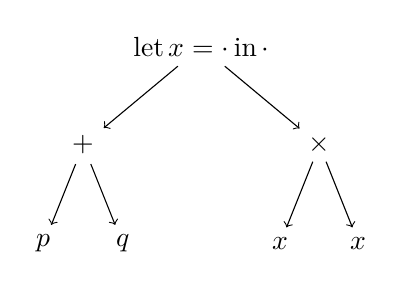
\begin{tikzpicture}
\node at (0, 2.5) (let) {$\mathrm{let}\,x=\cdot\,\mathrm{in}\,\cdot$};
\node at (-1.5, 1.25) (plus) {$+$};
\node at (-2, 0) (a) {$p$};
\node at (-1, 0) (b) {$q$};
\draw[->] (let) -- (plus);
\draw[->] (plus) -- (a);
\draw[->] (plus) -- (b);
\node at (1.5, 1.25) (times) {$\times$};
\node at (1, 0) (x1) {$x$};
\node at (2, 0) (x2) {$x$};
\draw[->] (let) -- (times);
\draw[->] (times) -- (x1);
\draw[->] (times) -- (x2);  
\end{tikzpicture}
  \caption{Abstract syntax tree}
\end{subfigure}%
\begin{subfigure}{.4\textwidth}
  \centering
\begin{tikzpicture}
\node at (0, 2.5) (times) {$\times$};
\node at (0, 1.25) (plus) {$+$};
\node at (-1, 0) (a) {$p$};
\node at ( 1, 0) (b) {$q$};
\draw[->] (times) to [out=240,in=120] (plus);
\draw[->] (times) to [out=300,in=60] (plus);
\draw[->] (plus) -- (a);
\draw[->] (plus) -- (b);
\end{tikzpicture}
  \caption{Term graph (with the let-binding inlined)}
\end{subfigure}
\caption{Comparising representations of \texttt{let x = p + q in x * x}}
\label{fig:term-repr}
\end{figure}

% dataflow computation

\subsection{Optimisations} \label{general-optimisations}

We briefly introduce typical compiler optimisations that are particularly important in this project.

Firstly, we summarise \textbf{common subexpression elimination} (CSE): whenever a program contains multiple computations of a pure expression $e$, we may instead introduce a variable $x$ defined to be $e$ and replace all existing occurrences of $e$ with $x$. Simple solutions include considering sets of subterms for each subterm and dominator trees. In the scope of this work, we consider a special case of CSE -- transformation of a term graph into an abstract syntax tree by insertion of let-bindings.

An important optimisation for a calculus with array comprehensions is flattening loops where nesting is unnecessary. When a subexpression does not depend on the state of the loop it is placed in, it may be computed before the loop starts. This is termed \textbf{loop-invariant code motion}, and can be performed via dataflow analyses.

\section{Requirements analysis}
\label{requirements-analysis}

As outlined in the Introduction and the Proposal, the project contains the following core deliverables:
\begin{itemize}
    \item \textbf{Formalisation} of a pointful array calculus, characterising what is expressible in the DSL.
    \item \textbf{Front-end embedding} of the DSL in Python, producing programs in the introduced calculus.
    \item \textbf{Execution back-end} for running programs efficiently by targeting existing array frameworks.
\end{itemize}
There were many possible variations on any of these points, so best judgements were made to fulfil the success criteria. A shallow embedding was chosen for the DSL, as it is an elegant approach that easily lends itself to metaprogramming in the host language. A major extension was the introduction of user-defined types in a way compatible with the DSL. The calculus was originally inspired by \textcite{paszke2021getting}, with extensions largely influenced by \textcite{shaikhha2019efficient} and focusing on improvements to the expressiveness and safety of the language. Lastly, since the paradigm does not possess particularly complex runtime features, a basic interpreter is easy to write. However, the goal of execution with the largest Python array programming framework -- NumPy -- was prescribed, so the scope of the calculus had to be adapted over time to the capability of the compilation technique. The execution method was intended to be generalisable to other array frameworks. No middle-end compiler phases were identified as a core deliverable, but they did form important extensions, including various compiler optimisations and program transformations.

\begin{center}
    \textcolor{purple}{TODO: Revise this section towards the end.}
\end{center}

\subsection{Methodology}

Owing to the modularity of the project and relatively orthogonal extensions, the \textit{spiral model} of development was adopted. After the initial milestones for each of the core deliverables (calculus, front-end, back-end), further ones focused on extensions. Priority was assigned based on impact on success criteria and practical usage, as well as efficiency of further work. Risk assessment relied on the existence of implementations or descriptions of a feature in the literature. Debug tooling for inspecting intermediate outputs is useful for debugging (particularly for a compiler), and as such it was also given priority.

\subsection{Review of array programs}
\label{suite-review}

Array programs vary significantly depending on the domain. One of these differences is in what language features are necessary to express them. For instance, deep learning programs rarely feature control flow, while differential equation solvers might perform iterated stencil computations. Even though application in deep learning is the original motivation, developing a more general calculus was preferable.

Due to my limited past experience with array programming applications, I conducted a comprehensive review of array programs. This assessment was conducted on the Futhark benchmark suite, with most programs classified based on their use of various language features, such as parallel programming patterns (reduce, scan, scatter), and the generality to which they are applied. In total, 29 cases were analysed, with the final language implementation being able to efficiently express most programs.
An example conclusion from this review was the inclusion of the sequential loop primitive (fold). It allows expressing many of the reviewed programs, which the original calculus could not. 
Furthermore, a majority of the evaluation benchmark suite is based on these cases. 

\subsection{Choice of language}

Python was chosen as the main language, as it is the host language for the DSL. This choice was made as it is a rather common choice for array programming generally. In particular, NumPy's first-class interface is in Python. Hence, the frontend and runtime were both fixed to Python. Only the middle/back-end could be moved to another language -- and one with a robust Python cross-language interface. 

A notable example of such a language is Rust. However, attempts at an early prototype showed a trade-off due to its restrictive type system. Though it could have ensured performance and reliability in the long run, it sorely slowed down development, especially when coupled with my relative inexperience. Alternative implementation languages included C++ which lacks features that simplify implementations of a high-level compiler, though it is a primary choice for Python interfacing. Another possibility was OCaml, which is good for implementing compilers, but problematic for interfacing with Python. 

As Python is not the best choice for writing a compiler, a modern Python version was used to take advantage of structural pattern matching introduced in version \texttt{3.10}. This significantly improved the code quality and programming experience. 

\subsection{Version control and testing}

The main version control system (VCS) applied for the project was Git. The repository was actively backed up to GitHub and also periodically to other devices. All write-ups were either done locally in a Git repository synced to GitHub, or on-line in an Overleaf project which was also synced to GitHub. This was deemed sufficient to high reliability standards of the services applied, with a local device never holding the only copy of a core artefact. 

Python's \texttt{pytest} testing framework was applied, which is a relatively standard choice that I was familiar with. Thanks to Python's nature it is highly dynamic, and features such as parameterised tests ensured consistency across all the compiler targets (backends) implemented throughout the course of the project. Code coverage could also be tested and achieved a reasonable score of 90\% (TODO: re-run).

Most of the code was statically typed with Python's type annotation facilities, as verified by \texttt{mypy}. It was run in addition to a linter (\texttt{ruff}) and autoformatters (\texttt{black} with \texttt{isort} and \texttt{pyupgrade}). All of the tools were run via \textit{pre-commit hooks}, which ensured a clean state of the repository at all times.

\subsection{Licences}

\textit{TODO: All software applied was open-source and permitted educational use: Python, NumPy, PyCharm, pytest, pre-commit hook stuff (mypy, black, ...), ...}

\section{Starting point}
\label{starting-point}

Prior to starting the project, I had a solid amount of experience in Python and NumPy -- in particular through the \textit{Scientific Computing} course. I had not designed or implemented a programming language before, though I had implemented a shallow-embedded DSL in Python. I had done a fair amount of reading of primary sources on array languages to establish the feasibility of the project. Material learnt in \textit{Semantics of Programming Languages} and \textit{Compiler Construction} was useful throughout the course of the project.

No implementation code was written prior to the start, though I experimented with some of the elements of the project (tracing and compilation schemes). No existing codebases were used as a basis. 
% \textit{Types}, \textit{Denotational Semantics}, and \textit{Optimising Compilers}

  \chapter{Implementation}

We consider this project to be the implementation of a compiler for a domain-specific language. Throughout this chapter, we follow compiler phases from the frontend to the backend. 
\begin{itemize}
    \item We first introduce the \textit{Phi calculus}, which formalises pointful array programs (Section \ref{phi-calculus}). We consider its syntax, type system, and semantics.
    \item In Section \ref{ein-dsl} we showcase the domain-specific language itself -- \textit{\textbf{Ein}}. We describe its deep-embedding in Python. Since we use an embedding, we do not need a classical parser. Ein's API builds up expressions in Phi, after which a complete program can be explicitly \textit{evaluated}.
    \item To evaluate the program, we have to \textit{compile} it. We describe the most important analyses and transformations which form the Ein compiler's middle-end in Sections \ref{compiler-analyses} and \ref{compiler-transformations} respectively.
    \item The key contribution of this work is the \textit{code generation} scheme. The \textit{Axial} applicative is introduced, underlying the connection between pointful and point-free array programming (Section \ref{escaping-the-pointless}). 
    \item We then define our compilation target for programs in the array programming model -- \textit{Yarr}, our point-free array calculus -- and show how we compile Phi to Yarr through Axials (Section \ref{codegen}). 
    \item Once the program is represented in Yarr, we interpret it through an \textit{execution backend}. We focus on the use of NumPy, but note the approach is general enough to work with PyTorch (Section \ref{execution-backend}).
    \item We wrap up the chapter with a repository overview in Section \ref{repository-overview}.
\end{itemize}
Throughout this section code snippets are excerpts from executable Python using Ein. 


\newpage
\section{Theory -- Phi calculus}
\label{phi-calculus}

We begin by introducing the functional \textbf{Phi calculus}, which is the theoretical basis for Ein. I outline the design choices I made, and how they relate to the real capabilities of array libraries.

\subsection{Syntax and design}

\newcommand{\philet}[3]{\mathrm{let}\,{#1}={#2}\,\mathrm{in}\,{#3}}
\newcommand{\phivec}[3]{\Phi\, {#1}[{#2}] \ldotp {#3}}
\newcommand{\phifold}[5]{\mathrm{fold}\,{#1}[{#2}]\,\mathrm{over}\,{#3} = {#4}\,\mathrm{by}\,{#5}}
\newcommand{\phipair}[2]{\left\langle {#1}, {#2} \right\rangle}
\newcommand{\phifst}[1]{\mathrm{fst}\,{#1}}
\newcommand{\phisnd}[1]{\mathrm{snd}\,{#1}}
\newcommand{\phisize}[2]{\mathrm{size}_{#2}\, {#1}}
\newcommand{\phiasserteq}[2]{\mathrm{assert}\,{#1}={#2}}

We define the syntax and primitives of Phi. It is largely similar to $\tilde F$, as introduced by \textcite{shaikhha2019efficient}.
\begin{align*}
e ::=&\quad \phivec{i}{e}{e} \quad|\quad e[e]   &\text{(array comprehension, indexing)} \\
|&\quad \phifold{x}{e}{x}{e}{e}  &\text{(indexed fold)} \\
|&\quad \phipair{e}{e} \quad|\quad \phifst{e} \quad|\quad \phisnd{e} &\text{(pair construction, projections)} \\
|&\quad \sigma(e, \dots, e) &\text{(scalar operator)} \\
|&\quad \phiasserteq{e}{e} \quad|\quad \phisize{e}{k} &\text{(equality assertion, size along axis } k \in \mathbb N \text{)} \\
|&\quad \philet{x}{e}{e} &\text{(non-recursive let binding)} \\
|&\quad x \quad|\quad i \quad|\quad c &\text{(variable, index, constant)}
\end{align*}
The introduction form for arrays is the indexed \textit{array comprehension} $\Phi$ (pronounced \textit{for}) -- for instance, $\phivec{i}{5}{i}$ is the array $[0, 1, 2, 3, 4]$. The elimination form is \textit{indexing} $a[i]$ ($i$-th element of $a$). Phi interprets multidimensional arrays as either scalars (zero-dimensional base case) or vectors of arrays. In that respect indexing is into the \textit{outermost} axis. 

The indexed fold facilitates a simple repeated iteration with an accumulator, and is closely related to the \texttt{loop} construct in Futhark. One can see $\Phi$ as perfectly parallel, while $\mathrm{fold}$ expresses sequential computation.

Examples of scalar operators $\sigma$ include arithmetic ($+$, $\times$, \dots) and logic ($\land$, $\lor$, \dots) operators. Array sizes are obtained with the $\mathrm{size}$ primitive -- if $e$ has shape $(n, m)$, then $\phisize{e}{1} = m$. We also include equality assertions to construct annotations for static analysis.

A crucial feature of Phi is the addition of a special kind of variable -- indices $i, j, k, \dots$ -- which live in a separate namespace. They are solely introduced in array comprehensions, and receive special treatment in both the type system and the compilation scheme. We use usual variables $x, y, z, \dots$ in all other cases.

For example, the following Phi term computes the (left-associative) sum $\sum_{i=0}^{n-1} a_i$ for a vector $a$:
$$ \phifold{i}{n}{x}{0.0}{x + a[i]} $$

\subsection{Type system}

\newcommand{\phifloattype}{\mathrm{Float}}
\newcommand{\phiinttype}{\mathrm{Int}}
\newcommand{\phinattype}{\phiinttype}
\newcommand{\phibooltype}{\mathrm{Bool}}
\newcommand{\phivectype}[1]{\Box{#1}}
\newcommand{\phipairtype}[2]{{#1} \times {#2}}

The type system of Phi is relatively straightforward, except for the handling of indices. Type constructors are unconstrained, and we allow arrays of pairs (missing from most array frameworks).
\begin{align*}
\kappa &::= \phifloattype \mid \phiinttype \mid \phibooltype & \text{(scalar types)} \\
\tau &::= \kappa \mid \phivectype{\tau} \mid \phipairtype{\tau}{\tau} & \text{(Phi types -- scalars, vectors, pairs)}
\end{align*}
The typing judgement $\Gamma; \Delta \vdash e : \tau$ is slightly non-standard due to the presence of indices. We use a separate environment for variables $\Gamma$ and indices $\Delta$. Consider the rules for array comprehensions and folds:
\begin{center}
    \begin{prooftree}[center=false]
        \hypo{\Gamma; \diamond \vdash n : \phinattype}
        \hypo{\Gamma; \Delta, i \vdash e : \tau}
        \infer2{\Gamma; \Delta \vdash \phivec{i}{n}{e} : \phivectype{\tau}}
    \end{prooftree} \quad
    \begin{prooftree}[center=false]
        \hypo{\Gamma; \diamond \vdash n : \phinattype}
        \hypo{\Gamma; \Delta \vdash a : \tau}
        \hypo{\Gamma, k: \phinattype, x: \tau; \Delta \vdash e : \tau}
        \infer3{\Gamma; \Delta \vdash \phifold{k}{n}{x}{a}{e} : \tau}
    \end{prooftree}
\end{center}
Other typing rules are relatively standard and carry through both $\Gamma$ and $\Delta$. Note that sizes and iteration counts are typed under $\Delta = \diamond$ -- i.e. neither can depend on a comprehension index. This ensures \textit{regularity} of the parallelism involved. Since an array size cannot depend on the index at which the defined element is placed, all arrays must remain rectangular. Similarly, since all iteration counts are the same across all array elements, the same computation is applied at each index. Hence, this does not type:
$$ \phivec{i}{5}{\phivec{j}{\textcolor{red}{i}}{i + j}} $$
Regularity is a beneficial property that ensures an efficient compilation scheme. We achieve it by a simple type check, which replaces a runtime check in Futhark, or the dependent type system in Dex. 
% TODO: Typing rules and semantics in appendix?

\subsection{Semantics}

\paragraph{Conditionals} Phi does not feature a dedicated conditional expression. We consider conditionals to be a ternary scalar operator instead, which we write $\mathrm{where}(c, t, f)$ (owed to the \texttt{numpy.where} primitive). As such, both branches are always evaluated regardless of the condition. This design choice follows as the array programming model has no real notion of a \textit{branching} array computation -- both cases are evaluated, as this ensures efficient vectorisation (SIMD processing). In hardware, the related notion is \textit{predication}.
% -- particularly in GPUs or in CPU conditional move instructions.

\paragraph{Out-of-bounds} Since ternary evaluate both branches, indexing operations that take place in either branch might end up out of bounds even when guarded. 
The Jax framework tackles a similar problem in the context of hardware accelerators, 
% and in the context of hardware accelerators the best solution seems to be to gracefully recover from the error by 
and tends to clip indices or impute a constant result. 
For simplicity, Phi clips indices into bounds.

\paragraph{Invalid arguments} We consider it to be a runtime error where a size or number of iterations is negative. We do not dwell on this, as the semantics could easily be modified to be exception-free.

\subsection{Embedding Phi in Python}
\label{embedding-phi}

We embed Phi in Python to allow constructing and validating terms in the frontend. Conceptually, Phi's grammar is a sum type. To implement this pattern in Python, we use a sealed abstract base class \texttt{AbstractExpr} with a child class for each case of \texttt{Expr}. To construct the term $\phivec{i}{4}{\phivec{j}{4}{i \cdot j}}$, we write:
\begin{center}
\begin{cminted}{python}
i, j = Index(), Index()
four = Const(Value(4))
table = Vec(i, four, Vec(j, four, Multiply((At(i), At(j)))))
\end{cminted}
\end{center}
It is easy to implement `incremental' type checking for Phi. 
To prevent the construction of invalid terms, constructors calculate a type based on the subterms. To facilitate this, we make use of intrinsically typed variables. 
Furthermore, instead of string-based variable names, we use Python object identities.


\section{Frontend -- Ein}
\label{ein-dsl}

\textbf{Ein} forms the programmer-accessible side of the project, and is implemented as the \texttt{ein} Python library. Unlike a traditional compiler, our frontend is not formed by a lexer or parser, but \texttt{ein}'s API. We overview Ein's features and its design as a purely functional, pointful array DSL.

\subsection{Embedding}

One of the main influences on the design of the embedding is Jax \cite{frostig2018compiling}, which lays out a solid foundation.
% for encapsulating expressions and building programs up by tracing. 
% This indirection can be seen as an instance of multi-stage programming, since the constructed program can have global optimisations applied to it before execution. 
DSL values transparently encapsulate an expression type (Section \ref{embedding-phi}).
A useful feature is that let bindings in the language are implicit and later recovered by the compiler.
% object identity is used to establish the same expression is reused, which can be seen as a safe approximation of \textit{hash consing}. 
For example, say \texttt{a} is an Ein value, in which case \texttt{a + a} indicates adding \texttt{a} to itself. 
Then \texttt{a} is reused in the compiled program rather than recomputed.

\subsection{Arrays}

% All Ein values 
% Nearly all operations in Ein take place on values of the \texttt{Array} type. These incrementally construct expressions in the underlying calculus via tracing. 
Similarly to Phi, Ein considers arrays to be defined recursively as either \textbf{scalars} or \textbf{vectors} of arrays. These correspond to the \texttt{Scalar} and \texttt{Vec[T]} classes. The methods of \texttt{Scalar} correspond to the scalar operators of Phi. These can be performed with operator overloading (as in \texttt{Scalar.\_\_mul\_\_} -- \texttt{a * b}) and methods (\texttt{Scalar.sin} -- \texttt{a.sin()}). On the other hand, \texttt{Vec} implements \texttt{Vec.\_\_getitem\_\_}, so that we can write \texttt{a[i]}. These are exemplified below, with type annotations added for clarity:
\begin{center}
\begin{cminted}{python}
a: Vec[Scalar]
b: Scalar = a[0].sin() * a[1].cos()
\end{cminted}
\end{center}
Both \texttt{Scalar} and \texttt{Vec[T]} have an \texttt{expr} attribute, and succeeding values have theirs lazily built up their corresponding Phi expression. For example: 
\begin{center}
\begin{cminted}{python}
b.expr == Mul(
    Sin(Get(a.expr, const(0))), 
    Cos(Get(a.expr, const(1)))
)
\end{cminted}
\end{center}

We further distinguish subclasses of \texttt{Scalar} corresponding to the Phi scalars -- \texttt{Int}, \texttt{Float} and \texttt{Bool}. At runtime, Ein represents \texttt{Int} with 64-bit signed integers, and \texttt{Float} with a double-precision floating point. Depending on the workload, often different variations of these are used, and e.g. type promotion rules are defined. Including more of such scalar types in both Phi and Ein would be straightforward.x

\subsection{Combinators}

The central part of Ein are the pointful, comprehension-style \textit{combinators}: \texttt{array} and \texttt{fold}. Anonymous functions, defined with the \mintinline{python}{lambda} keyword, are applied to facilitate introduction of new variables -- for instance, the index in an array comprehension. As such, \mintinline{python}{array(lambda i: i, size=5)} describes the Phi expression $\phivec{i}{5}{i}$. Further, the summation in $\philet{a}{\phivec{i}{5}{i^2}}{ \sum_{i=0}^{4} a[i]}$ is expressed with a \texttt{fold}:
\begin{center}
\begin{cminted}{python}
a = array(lambda i: i*i, size=5)
s = fold(0, lambda i, acc: acc + a[i])
\end{cminted}
\end{center}
We avoid explicit variable introductions by making use of the host language's lambda functions, in a manner similar to \textcite{atkey2009unembedding} and Jax. The explicit approach is taken surprisingly often for the drawbacks it has -- for instance in the SymPy algebra library or Taco. In the latter we have to write:
\begin{center}
\begin{cminted}{python}
i, j = pytaco.get_index_vars(2)  # explicit introduction
S[i, j] = A[i, j] + A[j, i]      # i, j still live afterwards. danger!
\end{cminted}
\end{center}
This is evidently flawed, as there is nothing guarding against the reuse of variables in the wrong scope. 

We have noted NumPy is a first-order interface, as its operations cannot be parameterised by functions. On the other hand, \texttt{array} and \texttt{fold} are closer to Second-Order Array Combinators, which are indispensable in Futhark. They are a major step up in Ein's expressive power.



\subsection{Size inference}

\textit{Size inference} allows omitting the size of arrays in some contexts. Consider the following computation:
\begin{center} 
\begin{cminted}{python}
array(lambda i: a[i] + b[i], size=a.size(axis=0))
\end{cminted} 
\end{center}
Say that the vectors $\texttt{a}$ and $\texttt{b}$ have the same size. Then with size inference we may omit the explicit \texttt{size}:
\begin{center} 
\begin{cminted}{python}
array(lambda i: a[i] + b[i])
\end{cminted} 
\end{center}
Specifically, for any index \texttt{i} that does not have an explicit \texttt{size} defined, it is inferred by taking the size of any array \texttt{a} that is indexed directly with \texttt{i} (i.e. in an expression \texttt{a[i]}), which we find by term graph traversal. Where there are other such candidates \texttt{b}, we add a program assertion that \texttt{a} and \texttt{b} have the same size. We further generalise this to the \texttt{fold} combinator, as its loop counter is often used to iterate over arrays.

% This is not as obvious to implement correctly as it seems at first sight. Due to the Phi typing rules, any sizes cannot (even indirectly) depend on a comprehension index nor on a value from an inner scope. Various simplifications and checks are performed to avoid bad candidates for an inferred array size.

There are many mechanisms similar to size inference, for instance in Single-Assignment C and in a more structured way in Dex via its value-dependent type inference. 
% In DSLs taking direct inspiration from Einstein summation, such approaches are often the only way of specifying array sizes. Ein also provides the flexibility of providing an explicit array size, as shown in the former example.

\subsection{Records}

So far, we have not yet described how Ein makes use of Phi's pair types. Indeed, in Ein we use them internally for representing labelled record types. We use a basic list encoding, where $\{ x: \phiinttype, y: \phifloattype, z: \phivectype{\phiinttype} \}$ becomes $\phipairtype{\phiinttype}{\left( \phifloattype \times \phivectype{\phiinttype} \right)}$. However, in contrast to \texttt{Vec} and \texttt{Scalar}, we do not use a custom Ein class for representing records as Python values -- instead, we use builtin container types. We summarise the values $v$ accepted and returned by Ein's API in Figure \ref{fig:ein-values}.

\begin{figure}
    \centering
    \begin{align*}
    v \quad::=&\quad 
    \text{\mintinline{python}{Scalar}}
    & \text{(scalars)} \\
    \mid&\quad
    \text{\mintinline{python}{Vec}}[v]
    & \text{(vectors)} \\
    \mid&\quad
    \text{\mintinline{python}{dict}}[\text{\mintinline{python}{str}}, v] 
    \,\mid\, \text{\mintinline{python}{tuple}}[v, \dots] 
    \,\mid\, \texttt{Dataclass}_v
    & \text{(records)}
    \end{align*}
    \caption{Values $v$ under which Ein's primitives are \textit{closed}, mirroring the type annotations in Section \ref{type-annotations}.}
    \label{fig:ein-values}
\end{figure}

Below is an illustrative example of Ein records:
\begin{center} 
\begin{cminted}{python}
# Array of dictionaries (records {x: int, y: int, z: int})
a = array(lambda i: {"x": i, "y": i*i, "z": i*i*i}, size=10)
# Indexing into a returns a dictionary with the same keys (record fields)
assert list(a[4].keys()) == ["x", "y", "z"]
assert a[4]["y"].eval() == 16
\end{cminted}
\end{center}
Arbitrary records consisting of Python tuples, dictionaries, and dataclasses\footnote{Dataclasses are Python constructs similar to Java records. We assume all the fields of the dataclass also hold Ein values.} can be used as array elements -- and these are reconstructed when indexing into these arrays, so that the programmer only sees Python containers of other Ein values rather than opaque objects. 
% The only dynamically-sized values are arrays, which are handled through the \texttt{Vec} class. 

Records enable a new style of array programming, unavailable in established Python array libraries. It is possible to describe composable array structures of custom data types and define operations on them. For instance, one could define an array of dual numbers\footnote{Dual numbers are similar to complex numbers, but instead of the imaginary unit $i^2 = -1$ we instead have a symbol $\varepsilon^2 = 0$. They are particularly useful in forward-mode automatic differentiation, and one could use them for this purpose in Ein.} with overloaded operators by using a dataclass:
\begin{center}
\begin{cminted}{python}
@dataclass
class Dual:
    real: Float
    eps: Float
    def __mul__(self, other: Dual) -> Dual:
        return Dual(
            self.real * other.real, 
            self.real * other.eps + self.eps * other.real
        )
a = array(lambda i: Dual(i, 1.), size=5)  # constructs Vec[Dual]
b = array(lambda i: a[i] * a[i])          # calls Dual.__mul__
\end{cminted}
\end{center}
In contrast, most renditions of the array programming model struggle to achieve this sort of composability, as they tend to just consider \textit{whole arrays of primitives}. In Python, at best one could sub-class an array type, but this would not compose as well. With records, we can define overloaded operations and reuse existing code through \textbf{duck typing}. Efficient representation of records is ensured via program transformations (described in Section \ref{aos-to-soa}). Record types in Ein are a \textbf{zero-cost abstraction}.

\subsection{Type annotations}
\label{type-annotations}

Ein classes are usable as Python type annotations. 
For instance, \mintinline{python}{a: Vec[Vec[Float]]} indicates \texttt{a} is an Ein matrix of floats. Thanks to this design, it is possible to use standard type checkers like \texttt{mypy} for \textbf{gradual typing} of Python programs using Ein. Some type errors -- like attempting to add a scalar and a vector, or indexing into a scalar -- may be discovered before runtime. Furthermore, type hints for records work on the same principle -- we previously wrote \mintinline{python}{v: Vec[Dual]} for a vector \texttt{v} of dual numbers. Indexing into \texttt{v} returns \mintinline{python}{v[i]: Dual}, which is known to have the fields \mintinline{python}{v[i].real: Float} and \mintinline{python}{v[i].eps: Float}.

% This is a significant advance over NumPy, where this sort of static type checking combined with user-defined data types is virtually impossible. Ein also prefers runtime type checking (as in Section \ref{embedding-phi}) prior to compiling the program and performing any large computations.


\section{Analyses}
\label{compiler-analyses}

We now describe the main analyses applied on Phi calculus, which facilitate further transformations and efficient code generation. Since Ein produces Phi term graphs, this is the main form on which we operate.

\subsection{Normalisation of high-level operations}

Phi does not perfectly correspond to efficient operations available in NumPy. For instance, to express a summation of a vector $a$ one might write $\phifold{i}{\phisize{a}{0}}{x}{0.0}{x + a[i]}$, while in NumPy a \texttt{sum} routine is available. Thus, it becomes reasonable to pattern-match on \textit{high-level operations} within Phi programs that are semantically equal to some NumPy routine.

However, this is hardly sufficient in more complex cases. For instance, $a[\max(i - 1, 0)]$ could be efficiently interpreted as a variation of:
\begin{center}
\begin{cminted}{python}
numpy.pad(a[:-1],               # skip final element
          (1, 0), mode='edge')  # pad 1 at start with first value
\end{cminted}
\end{center}
This example additionally illustrates how unwieldy NumPy's API can be at describing semantically simple operations. Nonetheless, how would we infer this is a combination of slicing and padding? My general approach is to apply a variation of \textit{normalisation by evaluation}. Phi terms are reflected into normal forms, which we can \textbf{compose} under a certain algebraic structure. Later, these can be reified into our array program representation (Section \ref{yarr}) by synthesising an appropriate semantically equivalent operation.

For example, let us consider indexing of the form $\phivec{i}{n}{x[a \times i + b]}$, where $(x, a, b)$ are expressions with no free indices. This essentially%
\footnote{
There are some caveats when indices go out of bounds. Nevertheless, let us presume it is easy to synthesise the array operations.}
corresponds to the slicing \texttt{x[b::a]} -- a subarray starting at index \texttt{b} and stepping by \texttt{a}.
The simplest approach would be to match on the syntax $a \times i + b$, but this is unstable with respect to small changes to the program (like $b + a \times i$, or $(a \times i + b) + b'$).
To resolve this, we appeal to the semantics of Phi and the algebraic structure of affine functions (see Figure \ref{fig:affine-normal-forms}). 
If for some $e[e']$ the item $e'$ has an \textit{affine normal form} $a \times i + b$, we can synthesise a slicing.

\newcommand{\norma}[1]{\llparenthesis \,{#1}\, \rrparenthesis}
\begin{figure}
    \centering
\begin{align*}
\norma{i} &= 1 \times i + 0 \\
\norma{c\times e} &= (c \times a) \times i + (c \times b)
& \text{if } \norma{e} &= a \times i + b \\
\norma{e + e'} &= (a + a') \times i + (b + b')
& \text{if } \norma{e} &= a \times i + b \\
&& \text{and } \norma{e'} &= a' \times i + b'
\end{align*}
    \caption{We write $\norma{e} = a \times i + b$ for the affine normal form of $e$ (if it exists). If an expression can be decomposed through matching on these cases, then we say it has the normal form.}
    \label{fig:affine-normal-forms}
\end{figure}

We generalise the normalisation to the following forms: \begin{itemize}
    \item `Clipped-shifts', which correspond to slicing and padding. The normal form is $\min(\max(i + c, l), u)$.
    \item Sums of generalised Einstein summations (tensor contractions). Thanks to linearity, these have an algebraic structure closed under addition, multiplication, and summation. Using this form, we can generate calls to matrix multiplication routines (through \texttt{numpy.einsum}). This could be generalised to semirings other than $(+, \times)$, in which case we could e.g. call GraphBLAS.
\end{itemize}

\subsection{Size equivalences}

To determine safety of some optimisations, we need to reason about sizes of arrays. We do this by introducing a simple \textit{term equivalence judgement~$\equiv$} (as in some dependent type systems), which allows safe approximation of when arrays must be of the same size. Example inference rules are given in Figure \ref{fig:term-equivalence}.

% TODO: Say it is/implement an e-graph?
In the implementation, we traverse the entire program term graph, matching on the rules and unifying equivalence classes accordingly. Unification is done on a disjoint-set data structure \cite{cormen2022introduction}. We perform this analysis after reduction to the struct-of-arrays representation (Section \ref{aos-to-soa}).

\begin{figure}[h]
    \centering
    $$
    \phisize{\phivec{i}{n}{e}}{0} \equiv n
    \quad
    \phisize{\phivec{i}{\cdot}{e}}{k+1} \equiv \phisize{e}{k}
    \quad
    \phisize{e[e']}{k} \equiv \phisize{e}{k+1}
    \quad
    (\phiasserteq{e}{e'}) \equiv e \equiv e'
    $$
    \begin{prooftree}
        \hypo{\phisize{e}{k} \equiv \phisize{e'}{k} \equiv n}
        \infer1{\phisize{\left( \phifold{i}{\cdot}{x}{e}{e'} \right)}{k} \equiv n}
    \end{prooftree}
    \caption{Example rules of the Phi term equivalence judgement $\equiv$. The last rule states that if the size of an accumulator $e$ is the same at the start and after an iteration $e \mapsto e'$, the final result also has the same size.}
    \label{fig:term-equivalence}
\end{figure}

% \textit{Using equality assertions to create an equivalence judgement between sizes. Used for determining safety to elide some indexing operations and that operations do not explode memory usage.} \todothis 

\section{Transformations}
\label{compiler-transformations}

\subsection{Outlining}

The term graph form produced by Ein is particularly useful when performing analyses, as not as much information has to be carried through in contexts. However, it is not an intermediate representation apt for generating executable code. It lacks information on where values used multiple times should be stored and when should they be computed. To address this, we convert the \textbf{term graph} into an \textbf{abstract syntax tree}. We refer to this process as \textit{outlining}. The goal is inserting appropriate let bindings to prevent recomputing expressions. Notably, \textit{inlining} corresponds to removal of the let bindings inserted by outlining. We perform it by directly substituting all bindings, returning the AST to the term graph form.

The two main techniques applied are \textbf{common subexpression elimination} and \textbf{loop-invariant code motion}. The former rewrites computations like $e + e$ to  $\philet{x}{e}{x + x}$. Meanwhile, the latter ensures that terms constant across loop iterations are computed before the loop, as in:
$$ 
\phivec{i}{n}{a[i] + \left( \phivec{j}{n}{2 \cdot b[j]} \right)[i]} \quad\leadsto\quad \philet{c}{\phivec{i}{n}{2 \cdot b[i]}}{\phivec{i}{n}{a[i] + c[i]}} 
$$
We consider both of these transformations to be a special cases of \textbf{let insertion}. In this approach, we determine the expressions which should be let-bound and where. For simplicity, we associate the possible locations with nodes in the term graph. Thus for each term $t$ we find a list of terms $t'$ to bind at $t$ -- meaning we rewrite $t \leadsto \philet{x}{t'}{\{x/t'\}t}$. Here, $\{x/t'\}$ replaces the \underline{term} $t'$ with $x$.

An important simplification of the problem setup is that Phi calculus is pure. 
% Let insertions in this manner of ``reverse-substitution'' preserve program semantics. A
We also make use of the property that all subexpressions are evaluated at least once. We further assume all loops iterate at least once.

\paragraph{Common subexpression elimination} We perform CSE via a standard method on term graphs, which is by application of \textbf{dominators}. Consider a graph in which there is an edge $t \to t'$ whenever $t'$ is a direct subterm of $t$. Then consider the immediate dominator $t^*$ of a term $t$ -- $t^*$ is the smallest term that contains all instances of $t$. Hence, we should let-bind $t$ at $t^*$. We perform this insertion for every non-atomic term $t$ for which $\mathrm{indeg}\,t > 1$ (i.e. it has more than one parent). This directly yields an AST.
% This common subexpression elimination produces an abstract syntax tree given any term graph.

We compute the immediate dominators with the \texttt{networkx} package, which has $O(n^2)$ time complexity in the worst-case. Since our term graphs are acyclic, there exist a well-known $O(n \log n)$ algorithm \cite{ramalingam1994incremental}.

\paragraph{Loop-invariant code motion} We tackle the problem of recomputing values invariant across loop iterations. We want to compute these prior to the loop (i.e. terms like $\Phi$ and $\mathrm{fold}$). Our approach relies on a simple tree traversal, keeping track of the outermost point at which a computation can be inserted so that it does not invalidate lexical scope constraints.

% CUT: Could give a listing instead
% Since after CSE we have an AST, we can perform a tree traversal on it. For each term $t$, there is a stack of loop terms that it is a subterm of, and we can update it as part of the traversal. Each of these loop terms $s_\ell$ (and any let-bindings inside) introduces a set of symbols $S_\ell$, so the stack induces a sequence $(S_1, S_2, \dots, S_k)$. Denote the free symbols in $t$ as $T$. We observe the following: if $\left( S_\ell \cup \cdots \cup S_k \right) \cap T = \emptyset$, then it is safe to let-bind $t$ prior to the loop $s_\ell$. On the other hand, $t$ will be computed the fewest times if it is moved to the outermost loop. Hence, we pick the minimum $\ell$ that preserves lexical scopes. We find and insert this let-binding for all non-atomic terms $t$.

A tricky part of the implementation is the ordering in which insertions are performed. Making the wrong choices results in scope errors or infinite terms. 
% However, a careful implementation avoids these issues. 
Lastly, there are cases in which bindings may become trivial (e.g. $\philet{x}{y}{e}$). To erase these, we perform \textbf{copy propagation} by inlining all trivial bindings.

\needspace{3em}
\subsection{Array-of-structs to struct-of-arrays}
\label{aos-to-soa}

A standard technique in array programming is the array of structs (AoS) to struct of arrays (SoA) transformation. The Ein compiler uses it to reduce away the arbitrary vector types to simple arrays of primitive types. This is crucial, as our compilation target -- NumPy,\footnote{Technically, NumPy does allow defining custom \texttt{dtype}s, but this feature is mostly intended for (de)serialising binary data. Similar features are nevertheless unavailable in other array libraries.} and array libraries generally -- lack support for arrays of composite types like pairs. Once we eliminate arrays of pairs, the only types $\tau'$ are given by:
\begin{align*}
\alpha &::= \kappa \mid \Box \alpha \\
\tau' &::= \alpha \mid \tau' \times \tau'
\end{align*}
Hence, $\tau'$ can only be tuples of arrays. This vastly simplifies compilation and runtime value representation. An AoS-to-SoA transformation is also applied in $\tilde F$ and Futhark, but it is not described in detail \cite{henriksen2017futhark, shaikhha2019efficient}. 

The isomorphism the operation relies on is $\Box (\tau_1 \times \tau_2) \cong \Box \tau_1 \times \Box \tau_2$, i.e. for each array of pairs there is an equivalent pair of arrays (of the same size). As such, we need only consider the introduction and elimination forms of arrays of pairs. The core transformation is depicted in Figure \ref{fig:aos-to-soa}.

\newcommand{\phisoa}[1]{\mathcal S \left\llbracket {#1} \right\rrbracket}
\newcommand{\phitupleindex}[2]{\mathcal P \left\llbracket {#1}, {#2} \right\rrbracket}

\begin{figure}
    \centering
    \begin{align*}
\phisoa {\phivec{i}{e_n}{e}}
&= \phipair{\phivec{i'}{\phisoa{e_n}}{\phifst{\phisoa{e}}}}{\phivec{i''}{\phisoa{e_n}}{\phisnd{\phisoa{e}}}}
&\text{(where }\Gamma; \Delta, i \vdash e : \phipairtype{\tau_1}{\tau_2} \text{)} \\[0.5em]
\phitupleindex{e}{e'}
&= \phipair{\phitupleindex{\phifst{e}}{e'}}{\phitupleindex{\phisnd{e}}{e'}}
&\text{(where }\Gamma; \Delta \vdash e : \phipairtype{\tau_1}{\tau_2} \text{)} \\
\phitupleindex{e}{e'}
&= e\left[ e' \right]
&\text{(where }\Gamma; \Delta \vdash e : \phivectype{\tau} \text{)} \\
\phisoa{e[e']}
&= \phitupleindex{\phisoa{e}}{\phisoa{e'}}
&\text{(where }\Gamma; \Delta \vdash e : \phivectype{\tau} \text{)} \\[0.5em]
\phisoa{e + e'}
&= \phisoa{e} + \phisoa{e'}
&\text{(and similarly for other cases)} \\[0.5em]
\phisoa{\phivectype{(\phipairtype{\tau_1}{\tau_2}})} &= \phipairtype{\phivectype{\tau_1}}{\phivectype{\tau_2}} &\text{(identity otherwise)}
    \end{align*}
    \caption{The core of the type-driven AoS-to-SoA transformation on Phi, denoted by $\mathcal S$. $\mathcal P$ maps an indexing to all arrays in the tuple. Environments $\Gamma; \Delta$ are passed through implicitly, in accordance with typing rules.}
    \label{fig:aos-to-soa}
\end{figure}

\section{Escaping the Pointless with Axials}
\label{escaping-the-pointless}

\textbf{Axials} are the key contribution of this work. They establish a new formal connection from pointful to point-free array programming. Thus, we can escape programming pointless (point-free) code by translating pointful code to it. Their structure is natural, in the sense that it forms an applicative functor.


\newcommand{\sizeat}[1]{s_{#1}}
\newcommand{\altsizeat}[1]{S_{#1}}
\newcommand{\denotindex}{\mathrm{Index}}
\newcommand{\denotvalue}{\mathrm{Value}}
\newcommand{\denotvar}{\mathrm{Var}}
\newcommand{\denotenv}{\mathrm{Env}}
\newcommand{\denotenvindex}{\mathrm{IndexEnv}}
\newcommand{\denotenvvar}{\mathrm{VarEnv}}


\paragraph{Motivation}
We shall use $A \simeq B$ to denote an isomorphism, where there exist a bijection between sets $A$ and $B$. To motivate Axials, we appeal to the separation of identifiers in Phi into variables $x, y, z, \dots$ and indices $i, j, k, \dots$. Hence, there is a similar separation of environments $\denotenv \equiv (\denotvar + \denotindex) \to \denotvalue$:
$$ \denotenv \simeq \denotvar \times \denotenvindex $$
Let us now consider the denotation of a Phi expression $e$, given by $\llbracket e \rrbracket : \denotenv \to \denotvalue$. We can now apply currying within the denotation:
$$\llbracket e \rrbracket : \denotenv \to \denotvalue \simeq \denotenvvar \times \denotenvindex \to \denotvalue \simeq \denotenvvar \to \boxed{\denotenvindex \to \denotvalue}$$
Functions $\denotenvindex \to \denotvalue$ turn out to have a lot of structure.
Since indices are only introduced in  comprehensions, we know their values must be within a range of integers like $i \in \left[ 0, \sizeat i \right)$
-- where $\sizeat i$ is the \textit{size} of an index $i$, as introduced in $\phivec{i}{\sizeat i}{e}$. 
This leads us to say that:
$$ \mathrm{dom}\,\denotenvindex \simeq \left[0, \sizeat i \right) \times \left[0, \sizeat j \right) \times \left[0, \sizeat k \right) \times \dots $$ 
where $\iota = \{i, j, k, \dots \}$ are the free indices in $e$.%
\newcommand{\denotarrayiota}{\mathrm{Array}_{|\iota|}}
Indeed, thisx \textit{index space} directly corresponds to that of a $|\iota|$-dimensional array of shape $(\sizeat i, \sizeat j, \sizeat k, \dots)$ -- the set of which we denote $\denotarrayiota$. 
The difference is that our `array' has \textit{labelled} axes, rather than \textit{positional} ones.
We denote $\iota!$ as the set of permutations of $\iota$.\footnote{Throughout this text permutations are \textit{orderings} of a set -- sequences where each element occurs exactly once. If $\iota = \{i, j, k\}$, then $\iota! = \{[i, j, k], [i, k, j], [j, i, k], [j, k, i], [k, i, j], [k, j, i]\}$.}
To complete the connection with arrays, we need to order our labelled axes:
$$ \denotenvindex \to \denotvalue \simeq \iota! \to \denotarrayiota $$
We have obtained that expressions of type $\tau$ dependent on indices $\iota$ can be evaluated as a $|\iota|$-dimensional array of $\tau$. We shall assume onwards indices are \textit{intrinsically sized}, meaning we have a constant $s_i \in \mathbb N$.% 
\footnote{This is merely a useful assumption to clean up the rest of the reasoning. Note that in general there is a unique Phi \textit{expression} which computes the size -- and this is what the compilation scheme relies on.}

We can finally substitute the result back into the type of $\llbracket e \rrbracket$:
$$ \boxed{ \llbracket e \rrbracket : \denotenv \to \denotvalue \simeq \denotenvvar \to \iota! \to \denotarrayiota } $$
We took the jump from pointful \textit{(given an assignment to each index, compute $\tau$...)} to point-free style \textit{(using an array of values $\tau$ at each possible index...)}. \textbf{Axials} are an encoding of $\iota! \times \mathrm{Array}_{|\iota|}$, fixing the ordered \textit{axes} and encapsulating the connection on the point-free side. We define this encoding so that it is natural, and thus composes well from subexpressions of $e$.
% \footnote{For instance, if $e = e' + e''$, then the axial $\denot e$ can be given in terms of $\denot {e'}$ and $\denot {e''}$}

\paragraph{Definition} 
We define an Axial to be the type constructor $\mathrm{Axial}\,\alpha \equiv \mathrm{List}\,\mathrm{Index} \times \mathrm{Array}\,\alpha$. Elements of the list component are called the \textit{axes} (they correspond to the ordering of free indices $\iota$ above), while the array is called the \textit{value} of the axial. We assume the number of dimensions in the value is the same as the number of axes; and each array axis has the same size as the index to which it corresponds.

We show Axials form an applicative functor. To this end, we need to define:\footnote{A complete proof would also show the definitions satisfy the \textit{applicative laws} (i.e. behave well under function composition).}
\begin{align*}
\mathrm{pure} &: \alpha \to \mathrm{Axial}\,\alpha \\
\mathrm{lift} &: (\alpha \to \beta \to \gamma) \to (\mathrm{Axial}\,\alpha \to \mathrm{Axial}\,\beta \to \mathrm{Axial}\,\gamma) 
\end{align*}
The former, $\mathrm{pure}$, is straightforward -- we can simply write:
$$ \mathrm{pure}\,a = \phipair{[]}{a} $$
On the other hand, to define $\mathrm{lift}\,f\,a\,b$, we need to think of an axial as a collection. We follow the formulation for $\mathrm{ZipList}$, which applies $f$ elementwise to $a$ and $b$:
$$ \mathrm{lift}\,f\,a\,b \sim \Phi\, i.\, f(a[i], b[i]) $$
We need to perform a similar operation in a \textit{axis-aware} manner. The idea may be illustrated as follows. Say we have axials $a = \phipair{[i, j]}{\texttt{a}}$ and $b = \phipair{[k, j]}{\texttt{b}}$ . We want to unify their axes (free indices), producing an Axial $c = \phipair{\gamma}{\texttt{c}}$. We \textit{choose} the axes $\gamma = [i, j, k]$, in which case $\texttt{c}$ is given by:
$$ \texttt{c}[i, j, k] = f(\texttt{a}[i, j], \texttt{b}[k, j]) $$
this is essentially an instance of \textbf{broadcasting}, solidifying a connection with point-free array programming.

Without going into detail (the Axial setup is a bit different in the compilation scheme) and with some abuse of notation, we define the following $\mathrm{lift}$ for axials $a = \phipair{\alpha}{\texttt{a}}$ and $b = \phipair{\beta}{\texttt{b}}$:
$$ 
\mathrm{lift}\,f\,a\,b = \phipair{\gamma}{\Phi\,\overline{\gamma}. 
f \left( \texttt{a}[\overline{\gamma}]_\alpha^\gamma, \texttt{b}[\overline{\gamma}]_\beta^\gamma \right) } \quad \text{where } \gamma = \alpha \sqcup \beta
$$
where $\gamma = \alpha \sqcup \beta$ deterministically picks some permutation of axes from both $\alpha$ and $\beta$, and $\Phi\,\overline{\gamma}$ constructs a multidimensional array with indices in $\gamma$ (and sizes consistent with \texttt{a} and \texttt{b}). 
Indexing into $a$ and $b$ respects the new axes $\gamma$, removing and permuting indices.

% \paragraph{Examples} 
% Take $\mathrm{mergeAxes}\,x\,y = \mathrm{sort}\,(\mathrm{concat}\,x\,y)$. \\ Set $a = \{ [i, j], \{i \mapsto 2, j \mapsto 3 \}, [[0, 1, 2], [3, 4, 5]] \} $, $b = \{ [j, k], \{ j \mapsto 3, k \mapsto 1 \}, [[0], [-1], [-2]] \}$. Then:
% $$ d = \mathrm{lift}_2\,(+)\,a\,b = \{ [i,j,k], \{i \mapsto 2, j \mapsto 3, k \mapsto 1 \}, [[[0], [0], [0]], [[3], [3], [3]]] \} $$
% Similarly, set $c = \{ [j, i], \{ j \mapsto 3, i \mapsto 2 \}, [[0, -2], [1, -1], [2, 0]] \}$, in which case:
% $$ e = \mathrm{lift}_2\,(-)\,a\,c = \{ [i, j], \{i \mapsto 2, j \mapsto 3 \}, [[0, 0, 0], [5, 5, 5]] \} $$
% Note that $e[i, j] = a[i, j] - b[j, i]$, hence $e[1, 2] = a[1, 2] - b[2, 1] = 5 - 0 = 5$. 

% It is helpful to consider the examples in the context of Phi. In the first, $d$ is evaluating the outer $+$ in $$\phivec{i}{3}{\phivec{j}{2}{\phivec{k}{1}{(3 \cdot i + j) + (j + k)}}}$$ in terms of the sub-expressions $3 \cdot i + j$ and $j + k$ (with Axials $a$ and $b$ resp.). In the second one, $e$ is computing the result of the subtraction in 
% $$\phivec{i}{2}{\phivec{j}{3}{(3 \cdot i + j) - \mathrm{where}(i = 0, j, 2 - j)}}$$ again in terms of the subexpressions. $e[1, 2]$ corresponds to the substitution $\{ i \mapsto 1, j \mapsto 2 \}$:
% $$ e[1, 2] = (3 \cdot 1 + 2) - \mathrm{where}(1 = 0, 2, 2 - 2) = 5 - \mathrm{where}(\bot, 2, 0) = 5 - 0 = 5 $$

\paragraph{Context} Why are Axials useful in relating different styles of array programming? Crucially, instances of $\mathrm{lift}$ are essentially just uses of NumPy-style \textbf{broadcasting}.
In fact, Axials can be seen as a generalisation of arrays. 
Instead of \textit{positional axes}, we have a notion of \textit{labelled axes}. 
This is reminiscent of recently introduced  \textit{named tensors} \cite{chiang2022named}. 
% In-memory representation still requires us to pick the axis ordering.

It turns out Axials relate to two well-known applicative functors -- the $\mathrm{List}$ and $\mathrm{ZipList}$. 
So far, we did not specify $\denotindex$ beyond assuming it has a notion of equality. 
It turns out that under the right $\denotindex$ we obtain (roughly) the behaviour of existing applicatives.
When we take $\denotindex \equiv \mathrm{Unit}$ we obtain the $\mathrm{ZipList}$, where $\mathrm{lift}$ always operates on lists elementwise.
% Any list can be converted to an Axial with the single axis, and $\mathrm{lift}\,f\,a\,b$ applies $f$ to respective pairs of elements in $a$ and $b$.
It is a well-known fact the $\mathrm{ZipList}$ cannot be generalised to a monad, thus there is no obvious Axial monad.
On the other hand, when $\denotindex \equiv \mathrm{Bool}$ we obtain the $\mathrm{List}$ applicative, for which $\mathrm{lift}$ operates on the cartesian product on lists. 
% For this construction, any application of $\mathrm{lift}$ needs to have the first operand along axis $\bot$, and the second along $\top$. 
% The result has both axes $\{ \bot, \top \}$, which we can convert back to a list by flattening -- thus applying $f$ for each pair in the cartesian product of $a$ and $b$.

\section{Code generation -- from pointful to point-free}
\label{codegen}

We now finally talk about how we can make the step from the pointful Phi calculus into the point-free array programming model. 
We devise \textit{Yarr} (a point-free array calculus), which is our target program representation. 
We show how Phi programs can be \textit{lifted} with the Axial, yielding a simple compilation scheme.

\subsection{Compilation target -- Yarr, the array calculus}
\label{yarr}

\begin{figure}
    \centering
    \begin{align*}
    \tau' ::=& \quad\kappa \mid \Box \tau' &\text{(arrays)} \\
    \tau ::=& \quad\tau' \quad\mid\quad \tau' \times \tau' \quad\mid\quad \dots &\text{(tuples of arrays)} \\
    E ::=&\quad \mathrm{range}(E)   &\text{(naturals up to }n\text{)} \\
    \mid&\quad \mathrm{size}(E, n)  &\text{(array size along axis)} \\
    \mid&\quad \mathrm{transpose}(E, (n, \dots)) &\text{(permute axes)} \\ 
    \mid&\quad \mathrm{squeeze}(E, n) &\text{(remove 1-axis)} \\
    \mid&\quad \mathrm{unsqueeze}(E, n) &\text{(add 1-axis)} \\
    \mid&\quad \mathrm{repeat}(E, E, n) &\text{(repeat along axis)} \\
    \mid&\quad \mathrm{gather}(E, E, n) &\text{(indexing along axis)} \\ 
    \mid&\quad \mathrm{elementwise}_\sigma(E, \dots) &\text{(elementwise op.)} \\
    \mid&\quad \langle E, \dots \rangle \quad\mid\quad \mathrm{proj}_n(E) &\text{(tuples and projections)} \\
    \mid&\quad \philet{x}{E}{E} &\text{(let-binding)} \\
    \mid&\quad \phifold{x}{E}{x}{E}{E} &\text{(indexed fold)} \\
    \mid&\quad x \quad\mid\quad c  &\text{(variables, constants)}
    \end{align*}
    \caption{The core of Yarr, our point-free array calculus. Operations are based on core NumPy primitives.}
    \label{fig:yarr-definition}
\end{figure}

We use a straightforward formalisation of point-free array programs for our compilation target, abstracting the interface of NumPy.
Figure \ref{fig:yarr-definition} shows the basic formulation into which we can compile Phi. It is extended with reductions, concatenation, specialised indexing operations (e.g. slicing), padding, and generalised Einstein summations. Note that the only significant common part with Phi is the indexed fold. 

In particular, indices $i$ from array comprehensions are erased entirely. The compilation scheme guarantees that no comprehension results in a fold. Otherwise, compiling Phi would be much easier -- one could set array elements one-by-one.

\needspace{5em}
\subsection{Compilation scheme}

\newcommand{\denot}[1]{\left\llbracket{#1}\right\rrbracket}

We now describe our scheme for compiling Phi into Yarr. It could be said it \textit{lifts} Phi expressions into the Axial applicative, at which point they are reified to computations in Yarr.

We introduce a transformation $\mathcal A \denot{e}$ mapping Phi terms $e$ to an Axial of Yarr terms $E$:
$$ \mathcal A \denot{e} = \langle \pi, E \rangle $$
where $\pi$ is a permutation of the free indices $\iota(e)$ of $e$. As with Axials, we call elements of $\pi$ the \textit{axes}. The encoding of $\mathcal A$ `flattens' the Axial \textit{values} -- and we set $\mathrm{rank}(E) = |\pi| + \mathrm{rank}(e)$. Thanks to the fact Axials form an applicative -- and hence are nicely behaved -- $\mathcal A \denot{e}$ can be composed from $\mathcal A$ for subterms of $e$. 

For a closed Phi program $p$, we shall expect that $P$ ($\mathcal A \denot{p} = \phipair{[]}{P}$) is its Yarr equivalent. It remains to fill in the gap where there are free indices (thus $\pi = \left[ \pi^{(1)}, \dots, \pi^{(k)} \right]$ is non-empty). We require the following \textit{semantic equivalence} property for $\mathcal A \denot e = \phipair{\pi}{E}$:
$$ \denot{\phivec{\pi^{(1)}}{\sizeat{\pi^{(1)}}}{\dots \phivec{\pi^{(k)}}{\sizeat{\pi^{(k)}}}{e}}} = \denot{E}$$
where $\sizeat i$ (in general, a Phi term) is used to denote the size of the range of index $i$. For example, consider $p = \phivec{i}{2}{\phivec{j}{3}{i + j}}$, so that $\sizeat i = 2$ and $\sizeat j = 3$. Then the following satisfies the property at $e \mapsto i + j$:
$$ \mathcal A \denot{i + j} = \phipair{[i, j]}{[[0, 1, 2], [1, 2, 3]]} $$

\newcommand{\sized}[1]{{#1} \triangleleft \sizeat{#1}}
We can now proceed to describe $\mathcal A$ for various Phi constructs. Firstly, we assumed that for any index $i$, we know the size $\sizeat i$. We achieve this by adding auxiliary Phi terms $\sized i$. Therefore:
$$ \mathcal A \denot{i \triangleleft \sizeat{i}} 
= \phipair{[i]}{ \mathrm{range} \left( \altsizeat{i} \right) }
\quad 
\text{where } \mathcal A \denot{\sizeat{i}} = \phipair{[]}{\altsizeat{i}} $$
To construct these auxiliaries, we substitute them at comprehensions (which introduce indices). Outside the comprehension body the index $i$ is no longer free, so we  remove $i$ from axes and adjust the encoding:
\newcommand{\dblsetminus}{\mathbin{{\setminus}\mspace{-5mu}{\setminus}}}
$$
\mathcal A \denot{\phivec{i}{\sizeat i}{e}} 
= \phipair{\mathcal \pi \dblsetminus i}{
\mathrm{transpose} \left( E, \theta_\pi^i \right)} 
\quad
\text{where } \mathcal A \denot{\{\sized i / i\} e} 
= \phipair{\pi}{E}
$$
where $\pi \dblsetminus i$ removes $i$ from $\pi$, and $\theta_\pi^i$ is the permutation that transposes the index $i$ onto the position of the outermost (Phi) axis. 
If $i$ was not free in $e$, we would use an appropriate $\mathrm{repeat}$ instead.

We now get to apply the Axial applicative. Constants $c$ are handled by $\mathrm{pure}\,c$ -- they have no axes:
$$ \mathcal A \denot{c} = \mathrm{pure}\,c $$
The other defining operation of an applicative -- $\mathrm{lift}$ -- also plays a central role. 
Take a scalar operator $e = \sigma(e_1, e_2)$, so that $\mathcal A \denot{e_1} = \phipair{\pi_{1}}{E_1}$ and $\mathcal A \denot{e_2} = \phipair{\pi_{2}}{E_2}$. 
We want to \textit{align} the results of $E_1$ and $E_2$ so that they have compatible axes $\pi$ which we can \textbf{broadcast} over. 
Indeed, $\pi$ needs to be a permutation of the indices $\iota(e_1) \cup \iota(e_2)$. 
This new choice of axes requires coercing $E_p$ ($p \in \{1, 2\}$) -- we need to first transpose $E_p$ (to match the order in $\pi$ from $\pi_{p}$), and then unsqueeze missing axes (the ones missing in $\pi_{p}$). 
We write $\pi = \mathrm{aligned}(\pi_{1}, \pi_{2})$ for choosing new axes, and the change-of-axes as $\mathrm{align}(E_p, \pi_{p}, \pi)$. The final formulation closely corresponds to a point-free $\mathrm{lift}\,\mathrm{elementwise}_\sigma$:
\begin{align*}
\begin{split}
&\pi = \mathrm{aligned}(\pi_{1}, \pi_{2}) \\
&E_1' = \mathrm{align}(E_1, \pi_{1}, \pi) \quad E_2' = \mathrm{align}(E_2, \pi_{2}, \pi) \\
&\mathcal A \denot{\sigma(e_1, e_2)} = \left\langle \pi, \mathrm{elementwise}_{\sigma}(E_1', E_2') \right\rangle 
\end{split}
% \tag{$\star$}
\end{align*}

We have covered the general technique on the core Phi constructs. We briefly overview the rest:
\begin{description}
    \item[Indexing] Indexing $e = e_1[e_2]$ is done in a very similar manner to elementwise operations through the $\mathrm{gather}$ operator, but the shape manipulation is a bit more involved. This is not exactly unexpected -- general indexing is notoriously difficult to express in NumPy.
    \item[Folds] Folds are an interesting case. Both the accumulator and the body have axes which need to be aligned (same as before). Since iteration counts are independent of indices $i$, the fold step is perfectly data-parallel, as we apply the same operation at each index. Due to fold's generality, at runtime we interpret them as \mintinline{python}{for} loop -- but its overhead is often dominated by the data-parallel iteration.
    \item[Tuples] After the SoA-to-AoS transform (Section \ref{aos-to-soa}), we need only consider tuples of arrays of primitives. The encoding is generalised to support them by prepending axes $\pi$ to each array in the tuple.  
\end{description}
It is worth note that throughout the encoding has been ambiguous -- due to the choice of \textit{axes} by $\mathrm{align}$. This choice has impact on performance -- it corresponds to the in-memory representation of the array. We use a deterministic heuristic to minimise the transpositions needed. 

% Compilation contract

\needspace{10em}
\section{Runtime -- Execution backends}
\label{execution-backend}

The compilation target of Ein is a high-level library in the array programming model. This means that most of the work is spent in large-workload whole-array operations, dominating the many overheads associated with Python. As such, we take some liberties to simplify the implementation. The primary technique we use is a (staging) function of the form
$$ \mathrm{Expr} \to \left( \denotenv \to \denotvalue \right) $$
where $\mathrm{Expr}$ is an expression in Phi or Yarr, and $\denotenv$ is a mapping from variables to assigned values. This essentially corresponds to directly implementing the denotational semantics $\llbracket e \rrbracket : \denotenv \to \denotvalue$ and composing the program from denotations of each subexpression $e$. We represent $\llbracket e \rrbracket$ with Python closures.

\subsection{Naive}

The first execution backend implemented was a \textit{na\"ive Phi interpreter}. It directly implements the denotational semantics of Phi, so Axial compilation is not necessary. 
% We still have to apply common subexpression elimination and loop-invariant code motion to avoid combinatorial explosion of the time complexity.
This backend was primarily used as a reference as time went on, as it was the easiest to extend. It focused on correctness rather than any notion of performance, and it is order of magnitudes slower than the NumPy backend. For example, staging $\phivec{i}{n}{2 \cdot i}$ results in a function \mintinline{python}{(dict[Variable, Value]) -> Value} equivalent to:
\begin{center}
\begin{cminted}{python}
lambda env: [2 * i for i in range(env[n])]
\end{cminted}
\end{center}

\subsection{NumPy}

We follow the same denotation-guided staging approach as in the naive backend. This time around we apply the whole suite of transformations and use Axial compilation from Phi to Yarr. The key difference is a stricter value representation that must rely on NumPy's \texttt{ndarray}s. We set values to be either arrays, or tuples of arrays. On this basis, we also apply some NumPy-specific performance optimisations.

\paragraph{Bindings} In some cases, NumPy attempts not to copy arrays, and instead returns a \textit{view}. For instance, \mintinline{python}{numpy.transpose(arr, (1, 0))} does not copy and instead returns an array with the same underlying data as \texttt{arr}, but a transposed layout. This is beneficial when the value is used once, but harmful when it is reused due to cache-inefficiency. We make use of a heuristic approach to address this -- whenever a view would be bound to a variable (hence reused), it is immediately copied to the target layout instead. 

Ein's let-bindings enjoy more efficient memory management than a manually-written NumPy program. In typical programs, new arrays are allocated sequentially. Afterwards, memory can only be freed by the garbage collector at the end of a function's scope. With explicit let bindings, we achieve higher granularity -- arrays can be freed as soon as they are no longer used.

\paragraph{Eliminating temporaries} Where they cannot return a view, NumPy operations allocate fresh memory for the result by default. Operations can be performed in-place instead, but idiomatic NumPy programs are inconvenient to write in this style (and thus waste memory). Consider adding three vectors \texttt{(a, b, c)}. The computation \texttt{a + b + c} will allocate memory for both \texttt{a + b} and \texttt{(a + b) + c}. If we can prove \texttt{a + b} will not be reused, we can reuse its memory. In NumPy, we would have to write:
\begin{center}
\begin{cminted}{python}
t = numpy.add(a, b)     # Allocate t = a + b
numpy.add(t, c, out=t)  # Reuse, update t := t + c
\end{cminted}
\end{center}
Ein's NumPy backend performs this in-place update optimisation automatically through a safe heuristic.
% which is more cache-friendly and saves needless memory allocations. 

\subsection{Generalising the NumPy backend}

\paragraph{Motivation} The very same methods as in the NumPy can be used in other array programming frameworks -- such as PyTorch, TensorFlow, and Jax. This is because they all derive from NumPy, as explained in the Preparation chapter. A PyTorch backend was implemented to test this in practice. PyTorch then efficiently executes programs on hardware accelerators (like GPUs), since it implements a suite of well-optimised \textit{kernels}. This showcases a general principle -- existing frameworks already implement hundreds of thousands of lines of performant code, and Ein can take advantage of this directly.

\paragraph{Automatic differentation} A feature common to all deep learning frameworks is the capability of performing \textit{automatic differentiation} (AD). Notably, we do not implement it directly in Ein. This choice is motivated by AD's availability in Ein's potential backends. Indeed, to differentiate an Ein function, we may use the PyTorch backend and make use of its existing facilities. In the following we compute $\frac{\partial \mathbf{a}^T \mathbf{b}}{\partial \mathbf{a}} = \mathbf{b}$:
\begin{center}
\begin{cminted}{python}
import torch
# Initialise a pair of vectors with gradient tracking
a, b = (torch.randn(3).requires_grad_(True) for _ in range(2))
# Compute a dot product in Ein and execute in PyTorch
c = reduce_sum(lambda i: wrap(a)[i] * wrap(b)[i]).torch()
# Run backpropagation through Ein's torch graph
c.backward()
return a.grad  # == b
\end{cminted}
\end{center}

\paragraph{Abstract backend} To facilitate addition of new backends, the \texttt{AbstractArrayBackend} interface was implemented. It declares a standard set of array routines, from which a Yarr interpreter may be derived.

\subsection{Extrinsics}

There are cases where Ein's compiler does not directly generate calls to functions available in the backend. For instance, \texttt{numpy.sort} would never get called directly by Ein. To this end, \textit{extrinsics} were implemented to facilitate calls to backend-specific functions. This is facilitated with the \texttt{ext} primitive, which takes a function and its Ein type signature. Extrinsics allow nearly-seamless integration of Ein and custom code, which vastly improves flexibility. In the below example, we sort an Ein \mintinline{python}{Vec[Float]} using \texttt{numpy.sort}:
% (the \texttt{sort} wrapper is unnecessary, but used for clarity):
\begin{center}
\begin{cminted}{python}    
def sort(x: Vec[Float]) -> Vec[Float]:
    return ext(numpy.sort, ([Vec[Float]], Vec[Float]))(x)
a: Vec[Float] = wrap(numpy.array([2.5, 0.0, 1.0]))
return sort(a).numpy()  # [0.0, 1.0, 2.5]
\end{cminted}
\end{center}

Ein does have to make some assumptions about the provided function, forming the \textit{extrinsic contract}. Firstly, the function has to be pure -- it cannot mutate its arguments. Secondly, it has to be broadcastable over additional leading axes of the arguments. Lastly, the shape of the array returned by the extrinsic must only depend on the shape of the arguments, ensuring arrays remain rectangular. 
% CUT
% On the example of \texttt{numpy.sort}: it works on a copy of the array; when called on a matrix it sorts the columns of that matrix (its last axis), broadcasting over the first axis; and it always returns an array of the same shape as its argument.

\section{Repository overview}
\label{repository-overview}

The Ein repository was built from scratch, and no pre-existing code was used.
It follows a usual Python project structure, with the root directory containing the \texttt{ein/} source directory, \texttt{tests/}, \texttt{tools/}, project configuration files (\texttt{pyproject.toml}, \texttt{.pre-commit-config.yaml}, etc.), and the Git configuration. 
A high-level breakdown is given in Table \ref{tab:repository}. The repository totals \todohere{} lines of Python code in the implementation and \todohere{} in the tests (as counted by \texttt{wc -l}, and the code formatted by \texttt{black}).

\begin{table}[h]
    \centering
    \begin{tabular}{c|c|l}
        Directory & Files & Description \\ \hline \hline
        \multirow{2}{*}{\texttt{ein/}} 
        & \texttt{debug.py} & Compiler debug utilities (e.g. \texttt{graphviz} diagrams) \\
        & \texttt{symbols.py}, \texttt{value.py}, \texttt{term.py} & Abstractions for defining Phi/Yarr \\ \hline
        \multirow{2}{*}{\texttt{ein/phi/}} & \texttt{phi.py} & Phi grammar and typing rules \\ 
        & \texttt{type\_system.py} & Type definitions \\ \hline
        \multirow{2}{*}{\texttt{ein/frontend/}} & \texttt{layout.py} & Encoding Ein records \\ 
        & \texttt{ndarray.py}, \texttt{comprehension.py}, \dots & Definitions of user-facing API \\ \hline
       \multirow{4}{*}{\texttt{ein/midend/}}       
        & \texttt{substitution.py} & Generic substitutions \\ 
        & \texttt{lining.py} & Inlining and outlining \\ 
        & \texttt{equiv.py}, \texttt{size\_classes.py} & Size equivalence judgements \\ 
        & \texttt{structs.py} & Array-of-structs to struct-of-arrays transform \\ \hline
       \multirow{3}{*}{\texttt{ein/codegen/}}       
        & \texttt{yarr.py} & Yarr grammar and typing rules \\ 
        & \texttt{axial.py} & Axials for Yarr \\ 
        & \texttt{phi\_to\_yarr.py}, \dots & Compilation scheme \\ \hline
       \multirow{3}{*}{\texttt{ein/backend/}}       
        & \texttt{naive.py} & Na\"ive Phi interpreter \\ 
        & \texttt{array\_backend.py} & Abstract array backend definition \\
        & \texttt{numpy\_backend.py} & Execution backends \\ \hline
       \texttt{tests/}       
        & \texttt{test\_*.py} & General and feature-specific tests \\ \hline 
       \texttt{tests/suite/}       
        & \makecell{\texttt{deep/*.py}, \texttt{misc/*.py}, \\ \texttt{parboil/*.py}, \texttt{rodinia/*.py}} & Longer programs \textit{(cases)} for tests and benchmarks \\ \hline 
       \texttt{tools/}
        & \texttt{benchmark.py} & Benchmarking utility \\ \hline 
        \texttt{.} & \texttt{pyproject.toml}, \dots & Project configuration files
    \end{tabular}
    \caption{Overview of the Ein repository.}
    \label{tab:repository}
\end{table}

  \chapter{Evaluation}

Following the project proposal, evaluation focused on \textbf{expressiveness}, \textbf{correctness} and \textbf{performance}.
As part of expressiveness, I consider Ein's usability as an alternative to NumPy, but also its computational limitations. For the latter criteria, I rely on diverse test and benchmark suites.

\section{Expressiveness}

We evaluate the expressiveness of Ein from two perspectives: \begin{itemize}
    \item For a \textit{programmer}, what patterns are easier to express in Ein than in the established NumPy?
    \item \textit{Computationally}, what can or cannot be expressed in Phi, Ein's formal program representation?
\end{itemize}

\subsection{Programming in Ein}

I argue that Ein is a superior alternative to NumPy-like array frameworks in a variety of cases. 
Ein's design takes advantage of the pointful style and higher-order combinators. 
It introduces language features unseen in the array programming model.
On the other hand, NumPy is occasionally more concise and is much more mature as software, but often leads to bad code for complex operations.
To illustrate the key points, we follow a few case studies and discuss the differences between Ein and NumPy implementations.

\subsubsection{Logits in a Graph Attention Network}

Our flagship example of an unwieldy many-dimensional operation is the logit computation in a Graph Attention Network (GAT), as introduced in the very first chapter. The NumPy implementation below was paraphrased from the original real-world Jax code (the interface of which is based on NumPy):
\begin{center}
\begin{cminted}{python}
def logits(att_1, att_2, att_e, att_g):
    return (
        transpose(expand_dims(att_1, axis=-1), (0, 2, 1, 3)) +  # + [B, H, N, 1]
        transpose(expand_dims(att_2, axis=-1), (0, 2, 3, 1)) +  # + [B, H, 1, N]
        transpose(att_e, (0, 3, 1, 2)) +                        # + [B, H, N, N]
        expand_dims(expand_dims(att_g, axis=-1), axis=-1)       # + [B, H, 1, 1]
    )                                                           # = [B, H, N, N]
\end{cminted}
\end{center}
We re-express this in the following Ein code:
\begin{center}
\begin{cminted}{python}
def batch_logits(s, t, e, g):
    return array(lambda h, u, v: s[u, h] + t[v, h] + e[u, v, h] + g[h])

def logits(att_1, att_2, att_e, att_g):
    return array(lambda b: batch_logits(att_1[b], att_2[b], att_e[b], att_g[b]))
\end{cminted}
\end{center}
It is worth remarking that the Ein code compiles into NumPy calls which are just as efficient as the base implementation. We move on to discuss the key differences:

\begin{description}
    \item[Shape manipulation] The array programming model revolves around manipulating array shapes to `align' them for subsequent whole-array operations. This does not generalise well to \textbf{many-dimensional data} -- the code becomes polluted with these manipulations (and \textit{axis indexing}), and hence syntax becomes unhelpful in determining the actual semantics. In contrast, Ein code relies on index-oriented descriptions. Extending the implementation with another dimension is just adding another index -- rather than modifying fragile arguments to NumPy routines. Additionally, index names serve to hint at the meaning of dimensions -- like variable names hint at data they store.
    % this is reminiscent of manipulating a program in a de Bruijin index representation, which is not convenient for a human.  
    \item[Batching] The Ein code is different from what was foreshadowed in the Introduction. We separated out \textcolor{blue}{\texttt{batch\_logits}}, which does most of the work, but disregarding the \textit{batch axis} (named \texttt{b}). A batch axis is a pervasive code structuring technique in NumPy code, which allows mapping an operation over many inputs (in our NumPy code comments denote it \texttt{B}). It is assumed that it will be carried through in broadcasting. In Ein, we explicitly map elements across each index \texttt{b}. This is clearer in intent and avoids arbitrary code conventions.
\end{description}

\subsubsection{Min-plus matrix multiplication}

We now consider the case of min-plus (or \textit{tropical}) matrix multiplication, which is relevant in shortest path problems. For a pair of matrices $A$ and $B$, its result is a matrix $D$ given by $D_{i,j} = \min_{k} A_{i,k} + B_{k,j}$ (like a usual matrix product, but in a $(\min, +)$ semiring instead of $(+, \times)$). We compare equivalently efficient NumPy and Ein implementations that compute this product in $\mathcal O(n^2)$ space.

\begin{center}    
\begin{minipage}[t]{.5\textwidth}
\raggedright
\begin{center}    
\begin{cminted}{python}
def min_plus_product(a, b):
    n,  m = a.shape
    m_, k = b.shape  # m == m_
    d = full((n, k), float("+inf"))
    for t in range(m):
      d = minimum(
        d, 
        expand_dims(a[:, t], axis=1) + b[t, :]
      )
    return d
\end{cminted}
\end{center}
\end{minipage}%
\begin{minipage}[t]{.5\textwidth}
\raggedleft
\begin{center}    
\begin{cminted}{python}

def min_plus_product(a, b):
    return array(
      lambda i, j: fold(
        float("+inf"),
        lambda k, acc: min(
            acc, 
            a[i, k] + b[k, j]
    )))

\end{cminted}
\end{center}
\end{minipage}
\end{center}

\begin{description}
    \item[Reasoning about shape] In this example, it is necessary to directly access NumPy array shapes to initialise the accumulator and compute the number of iterations. Code clarity requires introducing additional variables \texttt{n, m, k} to the code, disconnecting them from \texttt{a} and \texttt{b} which they describe. In Ein, \textbf{size inference} is sufficient to assign the right sizes and iteration counts in common cases.
    \item[Data-parallel loops] A space-efficient NumPy implementation necessitates a loop with a matrix accumulator. 
    % Using broadcasting instead would be more convenient, but would use excessive amounts of memory due to an intermediate cubic-size array. 
    Data-parallel loops like this are simple to express with Ein's \texttt{fold}. We avoid point-free reasoning about a matrix accumulator, instead focusing on a fixed index \texttt{(i, j)}.
    Arguably, the \texttt{fold} syntax is far from ideal, but readability could be helped with a shorthand:
    \begin{center}        
    \begin{cminted}{python}
def fold_min(f):
    return fold(float("+inf"), lambda k, acc: min(acc, f(k)))
d = array(lambda i, j: fold_min(lambda k: a[i, k] + b[k, j]))
    \end{cminted}
    \end{center}
\end{description}

\subsubsection{Pairwise $L_1$ distances}

In the last example, we compute the sum of absolute differences ($L_1$ distance) between every pair of rows of a matrix \texttt{A}. 
% This operation has the following index-oriented specification:
% $$ \texttt{pairwiseL1(A)}_{i,j} = L_1(\texttt{A}_i, \texttt{A}_j) = \sum_k \left| \texttt{A}_{i,k} - \texttt{A}_{j,k} \right| $$
We compare NumPy (as in \cite{maclaurin2019dex}) and Ein implementations:
\begin{center}    
\begin{minipage}[t]{.5\textwidth}
\raggedright
\begin{center}    
  \begin{cminted}{python}
def pairwiseL1(A: ndarray) -> ndarray:
  return sum(
    abs(transpose(A, (1, 0)) 
        - expand_dims(A, axis=2)),
    axis=1)
  \end{cminted}
\end{center}
\end{minipage}%
\begin{minipage}[t]{.5\textwidth}
\raggedleft
\begin{center}    
  \begin{cminted}{python}
def L1(u: Vec[Float], v: Vec[Float]) -> Float:
  return reduce_sum(lambda i: abs(u[i] - v[i]))

def pairwiseL1(A: Vec[Vec[Float]]):
  return array(lambda i, j: L1(A[i], A[j]))
  \end{cminted}
\end{center}
\end{minipage}
\end{center}
\begin{description}
    \item[Separation of concerns] The Ein implementation separates the computation of $L_1$ distances into the function \textcolor{blue}{\texttt{L1}} -- this is difficult to replicate in NumPy. By forcing reasoning on whole arrays, the array programming model actively discourages encapsulation. For example, say we want to generalise the code to different distances. A higher-order NumPy \textcolor{blue}{\texttt{pairwiseL1}} parameterised by the distance function would necessitate a certain contract (like a batch axis). In contrast, Ein's \textcolor{blue}{\texttt{pairwiseL1}} could be rewritten to take any distance function \texttt{dist} of the same signature as \textcolor{blue}{\texttt{L1}}:
    \begin{center}
    \begin{cminted}{python}
def pairwiseL1(A: Vec[Vec[Float]], dist: (Vec[Float], Vec[Float]) -> Float):
    return array(lambda i, j: dist(A[i], A[j]))
    \end{cminted}
    \end{center}
    Ein's user-defined types also lead to rich abstractions. For instance, it is possible to nearly replicate the automatic differentiation transformation of \textcite{shaikhha2019efficient} by implementing an appropriate dual number type. We benchmark the use of abstractions in the `Semirings' case (Section \ref{benchmarks}).
    \item[Type signatures] NumPy's support for useful type annotations is poor. Type checking with standard tools like \texttt{mypy} is even more problematic, and only partially solved by bespoke extensions \cite{liu2020type}. In contrast, Ein's type system is simple, behaves well under composition, and can be checked by \texttt{mypy}. For example, \texttt{mypy} infers the return type of \textcolor{blue}{\texttt{pairwiseL1}} -- \texttt{Vec[Vec[Float]]}. 
\end{description}

\subsection{Computation in Phi}

Having considered the practicalities of Ein, we consider its computational limitations on the basis of Phi. 
% We refer to known theory and features present in other array languages.

\paragraph{Primitive recursion} 
Phi is not Turing-complete -- all programs terminate. 
A lower bound on its expressive power is given by primitive recursive functions. 
Indeed, $\mathrm{fold}$ directly corresponds to primitive recursion $\rho$. 
Nevertheless, we argue Turing-complete computations are seldom necessary in array programming -- for instance, no native NumPy routines involve unbounded search. 
Since Ein is an embedded DSL, we can rely on the generality of its host language, Python -- as is standard practice. 

\paragraph{Lack of in-place updates} A major limitation of Phi is the lack of support for in-place updates (e.g. as in \mintinline{c}{a[5] = 42}). 
Since Ein is purely functional, we cannot simply rely on side effects to handle updates.
To this end, Futhark uses a uniqueness type system, while Dex makes use of an effect system \cite{henriksen2017futhark, paszke2021getting}. 

It is worth noting in-place updates can be (unsafely) replicated through the use of extrinsics as follows: 
\begin{center}    
\begin{cminted}{python}
def update(vec: Vec[Scalar], p: Scalar, x: Scalar) -> Vec[Scalar]:
    def with_update(arr: ndarray, pos: int, val: int) -> ndarray:
        arr[..., pos] = val; return arr
    return ext(with_update, vec.expr.type)(vec, p, x)    
\end{cminted}
\end{center}
Here, \texttt{update} mutates its \texttt{vec} argument, returning \mintinline{python}{array(lambda i: where(i != p, vec[i], x))}. Careless use leads to unexpected behaviour, but the approach exemplifies how extrinsics can be used to extend Ein.


\paragraph{Parallelism} Ein offers only limited support for common computational patterns. Though associative reductions were implemented as an extension, there are many other examples of useful parallel programming patterns. These are best exemplified by Futhark's array combinators -- particularly scan, histograms (\textit{scatter} in GPGPU programming), and filtering. Only some can be efficiently interpreted by calling out to NumPy routines, pointing to possible extensions to its interface.

\section{Correctness}

Formally proving the correctness of compilers is difficult, and few projects attempt it (e.g. CakeML \cite{kumar2014cakeml}). 
I settled for a robust test suite testing runtime correctness.

\subsection{Tests}

Ein's test suite (implemented in the \texttt{pytest} framework) mainly consist of compiled program output correctness in a variety of settings. 
I distinguish three kinds of such tests:
\begin{itemize}
    \item 13 Phi/IR-level tests. These consist of small program definitions directly in the Phi calculus. They are essentially unit tests for the na\"ive Phi interpreter.
    \item 59 Ein tests of small to medium length, which are implemented through Ein's API. This includes feature-specific tests for: extrinsics (4 tests), records (7 tests), and the PyTorch backend (6 tests).
    \item 9 \textit{case} tests, which are longer. They were constructed from publicly open array programs. We also use these for benchmarking (see Section \ref{benchmarks}).
\end{itemize}

Correct outputs are generated with Python reference code.
To obtain baseline outputs for Phi programs constructed by Ein I use the na\"ive Phi interpreter.
This allows diagnosis whether the problem is with the compiler to Yarr or the source Phi.
Outputs are treated as correct even when equality is approximate (with defaults of \texttt{numpy.testing.assert\_allclose}), as many tests use floating point arithmetic. 
Specifics of floating point semantics are often disregarded in domains like machine learning due to the limitations they cause in optimisations -- for instance, floating point addition is not associative \cite{alawi2004every}.

Most tests are parameterised by execution backend (through \texttt{pytest.mark.parametrise}) and run on random inputs. Since control flow in Phi is limited, random data is essentially sufficient to capture whether compiled programs behave correctly. 

The entire test suite passes successfully. The test line coverage across the implementation was measured to be \textbf{92\%}. Most of the untested code is in error paths, which were tested less often. Tests instead focus on ensuring that correct Ein/Phi programs behave correctly.
Checking that bad programs fail gracefully would mostly serve to test user experience, which was not part of the success criteria.

\subsection{Defensive programming}

To improve the capability of tests to pick up bad behaviour in internal parts of the implementation, a form of \textit{defensive programming} was applied throughout project code.
This was only a general practice of ensuring expected compiler invariants are met through Python \mintinline{python}{assert} statements. Failing an assertion generally indicates an internal compiler error and hence a bug. 

\needspace{2em}
We consider a few examples of this defensive approach: \begin{itemize}
    \item Types in the array-of-structs to struct-of-arrays program transformation are mapped in a consistent way ($\phisoa{\phivectype{(\phipairtype{\tau_1}{\tau_2}})} = \phipairtype{\phivectype{\tau_1}}{\phivectype{\tau_2}}$). We assert this mapping is upheld for each subexpression.
    \item Outlining asserts the original program $p$ and $\mathrm{inline}(\mathrm{outline}(p))$ are equal. Therefore, we ensure let-bindings inserted preserve program semantics.
    \item We check that all Phi and Yarr terms constructed within the compiler are well-typed.
\end{itemize}
% By testing invariants through program assertions and including feature-specific tests, a diverse component testing suite is formed. 

\section{Performance}

Ein's code-generation phase results in a Yarr program, which is by default interpreted by calling respective NumPy routines. 
Hence, our choice of compilation target (and runtime) is unique in the regard it is rather high-level.
The `machine instructions' are NumPy routines, and hence the we are limited by its performance. 
We rely on the established approach of comparing compiler-generated programs to baselines.
\subsection{Benchmarks}

\label{benchmarks}

We form a varied suite of baseline Python programs using NumPy (\textit{NumPy programs} for short). 
We then compare the baseline performance against equivalent Ein code.
The choice of our benchmark baselines is inherently subjective -- for any Ein-generated program using NumPy, there is a just-as-fast program using NumPy directly.
For a fair comparison, I aimed for \textit{idiomatic} NumPy code (e.g. freely allocating temporary arrays instead of managing memory).
We consider Ein to be \textit{efficient} if at large problem sizes the running time is within a small constant factor of the baseline. 


\begin{table}[b]
    \centering
    \begin{tabular}{c|c|l}
       \textbf{Benchmark} & \textbf{Source} & \textbf{Description} \\ \hline
        Attention & Open-source & core part of Neural Attention \\
        GAT & Open-source & inference in the Graph Attention Network architecture \\
        Semirings & Based on \textcite{dolan2013fun} & shortest paths via closure of a tropical semiring matrix \\
        MRI-Q & Parboil & basic linear reduction \\
        Stencil & Parboil & basic 3D stencil \\
        Hotspot & Rodinia & complex 2D stencil \\
        Pathfinder & Rodinia & 1D dynamic programming 
    \end{tabular}
    \caption{Brief overview of each of the Ein benchmark cases. They are also included in the test suite as system tests.}
    \label{tab:benchmarks}
\end{table}


\paragraph{Suite} Our benchmark suite (Table \ref{tab:benchmarks}) builds on the findings from Section \ref{suite-review}. 
Most cases are sourced from Futhark benchmarks \cite{The_Futhark_Hackers_futhark-benchmarks} (as done by Dex) and open-source implementations of deep learning architectures.
I hand-translated all of the cases from the source language (Futhark, or Python using PyTorch/Jax) into equivalent a pair of programs in Python using Ein or NumPy.

A benchmark case worth special note is \textit{Semirings}, which was implemented from scratch. 
The NumPy baseline is a standard $\mathcal O(n^3)$ implementation of the Floyd-Warshall all-pairs shortest paths algorithm. 
In Ein, I instead make rich use of arrays of user-defined dataclass types. 
I follow the approach of \textcite{dolan2013fun} for solving a general family of problems via matrices over \textit{closed semirings}%
\footnote{A \textit{closed semiring} is an algebraic structure following certain algebraic laws.
From an implementation perspective, they are a type which defines some closed binary operations ($+$, $\times$, and closure) and constants ($0$, $1$).
They are a useful abstraction -- for instance, the \textit{tropical semiring} turns out to capture shortest paths in a graph \cite{lehmann1977algebraic}.}.
I implemented his generic approach in Ein, taking advantage of efficient array operations.
% By implementing the \texttt{Tropical} instance of a \texttt{Semiring}, we can compute the closure of a generic \texttt{SemiringMatrix}, yielding the shortest paths.
NumPy lacks similarly capable abstractions, and in Ein we show they are of zero cost.
See Figure \ref{fig:semirings} for the crux of the generic Ein implementation.

\begin{figure}
    \centering
\begin{cminted}{python}
class SemiringMatrix:
    ...
    def closure(self):
        return SemiringMatrix(fold(
            self.elem,
            lambda k, acc: array2(
                lambda i, j: acc[i, j] + acc[i, k] * acc[k, k].closure() * acc[k, j]
        ).assume(self.elem[k, k]))) + self.one
\end{cminted}
    \caption{Closure of a \texttt{SemiringMatrix} in Ein (Algorithm 6.1 \cite{abdali1985transitive}). \texttt{+}, \texttt{*} are overloaded \texttt{Semiring} operations. When \texttt{+} is $\min$ and \texttt{*} is $+$, this reduces to the Floyd-Warshall shortest paths algorithm.}
    \label{fig:semirings}
\end{figure}

It is worth note that the other two cases used in the test suite -- NN and KMeans (from Rodinia) -- were excluded from the benchmark. A computationally efficient implementation of these relies on features unavailable in Ein (respectively in-place updates and histogram computations). They could be mimicked through extrinsics in practice, but their use would not constitute a useful benchmark.

\paragraph{Methodology} Benchmarks were conducted on an M1 Pro MacBook (14-inch, 2021). The versions used were CPython \texttt{3.11.6} and NumPy \texttt{1.26.4}. No further thread parallelism was used beyond what is used by default in NumPy (in linear algebra routines). Large problem sizes are used (about $1\,\mathrm{s}$ of execution time), taking the minimum time across at least 5 runs. Minimum time is used as each benchmark performs the same number of operations per run, so most overheads are caused by external factors. Ein's compilation time was not included in the measurement, but it is on the order of $2\,\mathrm{ms}$ and thus negligible.

\begin{figure}[b]
    \centering

    \pgfplotsset{
    /pgfplots/baseline legend/.style={
    legend image code/.code={
    \draw[thick,draw,color=red](-0.05cm,0cm) -- (0.3cm,0cm);%
       }
      }
    }
    \begin{tikzpicture}
        \begin{axis}[
            ybar,
            ymin=0,
            ymax=2,
            extra y ticks = 1,
            extra y tick labels={},
            extra y tick style={grid=major,major grid style={thick,draw=red}},
            symbolic x coords={Attention, GAT, Semirings, MRI-Q, Stencil, Hotspot, Pathfinder},
            legend entries={Ein, Baseline},
            xtick=data,
            ylabel={runtime/baseline},
            bar width=1.8em,
            width=\linewidth,
            height=13em,
        ]
    
        \addplot[draw=blue, fill=blue!30] coordinates {
            (Attention, 0.68) 
            (GAT, 0.75) 
            (Semirings, 0.67)
            (MRI-Q, 1.0) 
            (Stencil, 1.5)
            (Hotspot, 0.99)
            (Pathfinder, 1.16)
        };
        \addlegendentry{Ein}
        \addlegendimage{baseline legend}
        \addlegendentry{Baseline}
    
        \legend{Ein, Baseline}
        
        \end{axis}
    \end{tikzpicture}

    \caption{Ratio of the running time of Ein-generated NumPy programs, and the baseline NumPy. \textit{Lower is better.}}
    \label{fig:benchmark-results}
\end{figure}


\paragraph{Discussion} Benchmark results can be seen in Figure \ref{fig:benchmark-results}. 
We reach our efficiency goal -- Ein is no more than 60\% slower than the baseline, and in some cases it is up to 40\% faster.
Ein's is able to perform various optimisations -- eliminating allocations of temporary arrays is especially influential. 
On the other hand, performance deficits are especially due to missing advanced indexing strategies -- particularly in Stencil.
However, the baseline Stencil implementation is ridden with error-prone expressions. 
It contains nearly a dozen complex indexing expressions like \mintinline{python}{A[1:-1, :-2, 1:-1]}, which in Ein end up translated to forms like \mintinline{python}{A[x, y - 1, z]}.
Therefore we conclude Ein offers a good trade-off on code readability and performance.


\section{Work completed}
\label{work-completed}

We summarise the work completed basing on the success criteria from the proposal: \begin{description}
    \item[Designing a pointful array calculus] Phi was designed successfully, and ended up building on the $\tilde F$ language due to \textcite{shaikhha2019efficient}. This further includes various extensions with respect to the proposal: fully-fledged pair types, size assertions, folds, and associative reductions.
    \item[Embedding an array language in Python] The implemented \texttt{ein} library successfully embeds a pointful array language -- Ein -- in Python. Ein's API builds up terms in the Phi calculus, after which it allows calling out to the compiler to evaluate the program with an execution backend. Key extensions on the proposed core interface are: size inference, general \texttt{fold} and \texttt{reduce} combinators, extrinsics, rich record types, and support for type annotations.
    \item[Efficient execution backend] We compile pointful array programs (in the Phi calculus) by generating point-free array code (Yarr calculus) using the foundation of the newly introduced Axials. Yarr programs are efficiently interpreted by calling NumPy routines. A key extension was the inclusion of a PyTorch backend, taking advantage of hardware acceleration and automatic differentation.
\end{description}
Ein's compiler middle-end was also suitable for extensions: the array-of-structs to struct-of-arrays transformation and outlining (common subexpression elimination and loop-invariant code motion).


\needspace{2em}
\section{Summary}

Throughout this chapter we have seen that Ein is expressive, and can be superior in usability as an alternative to NumPy. 
It further has various language features unseen in NumPy-like frameworks.
Furthermore, robust tests ensure correctness of our implementation. 
Benchmarking has shown our execution backend is efficient on a varied suite of cases. 
Ein leads to much clearer programs than what would be written by a NumPy programmer, while preserving -- or even improving -- performance. 

  \chapter{Conclusions}

The project was a complete success. 
I have met all of the success criteria, and greatly expanded upon them with various extensions. 
I introduced novel techniques that reconcile colossal engineering efforts on the array programming model, and the promises of the pointful array programming paradigm. 
I also embedded several language features in Python one might not expect to be possible with existing array libraries. 
Due to Python's dominant role in machine learning and scientific computing, my techniques can be adapted to this ecosystem. 
On this basis, Ein represents an advance of array programming in Python.


\section{Research contribution}
\label{research-contribution}

I submitted papers on the topic of this project to two venues -- the ACM Student Research Competition at POPL (November -- January), and the ARRAY workshop at PLDI (March -- April).

\subsection{Student Research Competition}

The ACM Student Research Competition (SRC) consists of two stages -- the conference stage, and the Grand Finals for winners at each conference. In November I submitted a 3-page extended abstract to the SRC at the 51st ACM SIGPLAN Symposium on Principles of Programming Languages (POPL).
I received positive reviews and an invitation to present my work in January. 
There, I gave poster and oral presentations.
Throughout the entire process I was supported by my supervisor.
My work won \textbf{first prize} among undergraduates there. I was then invited to submit a 5-page extended abstract to the Grand Finals. Results for this stage are due later in May.

\subsection{ARRAY Workshop}

The ACM SIGPLAN International Workshop on Libraries, Languages and Compilers for Array Programming (ARRAY) concerns all aspects of array programming. 
This includes topics particularly relevant to this project: language design, embedded DSLs, paradigms, and compilation schemes.
ARRAY is colocated with the ACM SIGPLAN Conference on Programming Language Design and Implementation (PLDI).

As part of the proceedings of the workshop, together with my supervisor we authored a 12-page research paper on my work in early April. I wrote the main content, with my supervisor taking an advisory role. 

% TODO: Comment on results in late April.

\needspace{2em}
\section{Lessons learnt}

Ein was by far the longest-running software project I have worked on, and the first one which involved a significant theoretical and technical background. 
It was necessary to study the relevant concepts in programming languages and compilers.
Having worked with large codebases prior, the software engineering aspect did not pose as much of a challenge to me. 
On the other hand, designing Ein -- and the fundamentals underlying it, Phi and Yarr -- was far from straightforward. 
Furthermore, explaining and writing about my design also proved challenging. 

\subsection{Designing programming languages}

Ein sought to be a domain specific language for array programming -- targeting practical use in areas like machine learning -- embedded in Python. Each of these constraints posed problems.

\begin{description}
    \item[Domain-specific language] 
    Learning to choose the right \textbf{trade-offs} for my DSL was a major difficulty. 
    Whenever I thought ``should I introduce this feature?'' I was constrained by thinking how much it would impact the rest of the language and the compilation scheme. 
    I had to learn to make careful choices -- for instance including a basic loop primitive (\texttt{fold}) rather than a general while-loop -- led me to an efficient compilation scheme (in this case preserving regular data parallelism).
    \item[Array programming] 
    It was important to relate my project goals with what \textit{ought to be} possible in the language in the eyes of a domain practitioner. 
    To this end, I sought feedback of my colleagues in machine learning, and consulted external resources that distilled the benefits and drawbacks of the array programming model. 
    This taught me how to reconcile real-world use and language design.
    \item[Embedding in Python] 
    Python was not explicitly designed to host embedded DSLs. 
    Though it is extremely flexible (it is dynamically typed, interpreted and allows introspection), some design choices leave it constrained. 
    This is particularly in two main areas (where Python DSLs often fail) -- lack of flexible function overloading and variable introduction. 
    Finding a way to include new syntactic features that would be idiomatic \textit{(Pythonic)} was another source of trade-offs.
\end{description}

\subsection{Expressing ideas}

Throughout this project I explored many different ideas for language features. 
Unfortunately, I often lacked the necessary background to give them solid theoretical foundation. 
While implementation was a matter of software engineering, formalising ideas and communicating them across was challenging. 

Throughout the project, under encouragement of my supervisor, I submitted papers about my project to two venues (Section \ref{research-contribution}). 
This forced me to reflect on my ideas and find ways of explaining them succinctly.

\section{Future work}

Avenues for further work include:
\begin{description}
    \item[Generalising the compilation scheme] Can the Axial compilation scheme be further generalised to other combinators than array comprehensions, folds and associative reductions? Is it possible to integrate elements of irregular parallelism or jagged (non-rectangular) arrays?
    \item[Alternative backends] Is it beneficial to compile Phi to a different representation than Yarr? Though Yarr can be consumed by a framework like Jax and passed to a specialised linear algebra compiler like XLA, this loses out on some information. Can we take advantage of methods described for Dex and $\tilde F$ in the context of Python and Ein by implementing different execution backends \cite{shaikhha2019efficient, paszke2021getting}?
    \item[In-place updates] What is the best way of implementing safe in-place updates in the context of an embedded DSL? How can they be efficiently integrated with Ein's compiler, and what are good syntactic representations? Both Futhark and Dex offer some possible solutions \cite{henriksen2017futhark, paszke2021getting}.
\end{description}

%TC:ignore

  \appendix 

  % \chapter{Project Proposal}
  % \chapter{Project Proposal}

\newcommand{\dontcite}[1]{}

\textit{The following is quoted verbatim. However, formatting and citations were adjusted to be consistent with the rest of this document.}

\section{Introduction}

Tensors are an ubiquitous abstraction in the area of machine learning. In this context, they are $n$-dimensional arrays specialised for high-performance data parallel computing. The Python programming language dominates the machine learning research scene. However, its runtime overheads are far too high for the data processing to be expressed directly in the language. As such, Python highly benefits from the tensor abstraction with a set of highly optimised operations. This gave rise libraries and frameworks such as NumPy \cite{harris2020array}, PyTorch and TensorFlow.

These aforementioned libraries all share a common core of the \textit{array programming model}, as introduced in APL \cite{iverson1962programming}. The model is characterised by first-class multi-dimensional arrays. Primitives are parameterised in nontrivial ways, acting on the arrays as a whole -- individual elements are rarely referenced. The core benefit of this approach is that the implementations of individual primitives -- referred to as \textit{kernels} -- can be highly optimised (and written in another language). Programs in the model can also be surprisingly concise, as can be seen on Figure \ref{fig:pairwise-l1-numpy}. 

\begin{figure}[h]
    \centering
    \begin{minipage}{0.65\textwidth}
    \begin{minted}{python}
def pairwiseL1(a):
    return sum(abs(a.T - a[..., newaxis]), axis=1) 
    \end{minted}
    \end{minipage}
    \caption{Computing a matrix of pairwise $L_1$ distances between rows with axis manipulation and broadcasting in NumPy -- as given by Dex authors \cite{maclaurin2019dex}}
    \label{fig:pairwise-l1-numpy}
\end{figure}

Despite its widespread use in today's scientific computing and machine learning workflows, the array programming model is not without its problems. The available operations expose features such as broadcasting, which allow high expressiveness without sacrificing performance. However, these features also make programs difficult to write, debug and maintain \cite{paszke2021getting}. They are also nontrivial to statically analyse due to being highly dynamic, as the behaviour of operators may vary based on the shapes and element types of their inputs \dontcite{liu2020type}. This causes the need for comments in the host language, as few facilities exist for type annotations \dontcite{Rush2018}. Additionally, the actual implementation in terms of the available kernels may be distant from the mathematical description of a computation -- as can be seen in Figure \ref{fig:pairwise-l1-math}. The choice of kernels is not obvious, as their number is usually in the hundreds. More involved pieces of logic have to be expressed with more specialised kernels (if they exist), or otherwise complex  combinations of existing ones (suboptimal performance), or worst of all expressed directly in Python, which significantly hurts performance.

\begin{figure}[h]
    \centering
    $$ \texttt{pairwiseL1}(A)_{i,j} = \sum_{k} \left| A_{i,k} - A_{j,k} \right|  $$
    \caption{An index-oriented mathematical formulation of \texttt{pairwiseL1} from Figure \ref{fig:pairwise-l1-numpy}}
    \label{fig:pairwise-l1-math}
\end{figure}

All in all, these shortcomings cause novel deep learning architectures to be unreasonably difficult to express and optimise in the array programming model. This invites the exploration of new array programming paradigms which seek to solve these problems.

Dex \cite{paszke2021getting} is a recent research programming language implementing \textit{pointful} (or \textit{index-oriented}) array programming, which can be seen as a generalisation of \textit{Einstein summation notation}. Its distinctive feature is the \texttt{for} primitive, where an array's elements may be defined in terms of their indices. Programs written with this approach boast closeness to mathematical notation (Figure \ref{fig:pairwise-l1-dex}). Index bounds are inferred as in Einstein summation for clarity. Dependent types fulfil a central role for statically analysing array sizes. Dex demonstrates that the paradigm can achieve performance comparable to other approaches, such as the \textit{array-combinator} language Futhark \cite{henriksen2017futhark}.

\begin{figure}[h]
    \centering
    \begin{minipage}{0.6\textwidth}        
    \begin{minted}{haskell}
def pairwiseL1 (a : m=>n=>Float) : n=>n=>Float =
    for i. for j. sum for k. abs (a.i.k - a.j.k) 
    \end{minted}
    \end{minipage}
    \caption{Computation of \texttt{pairwiseL1} from Figure \ref{fig:pairwise-l1-numpy} in Dex}
    \label{fig:pairwise-l1-dex}
\end{figure}

However, application of an entirely new language like Dex poses further problems, such as its usability in the existing ecosystem. Embedding the DSL \cite{gibbons2014folding} is a popular approach to address this. Jax \cite{frostig2018compiling} can be seen as a domain-specific language within a shallow embedding in Python. Operations performed on Jax arrays are \textit{traced} into a staged expression. That IR can then be e.g. differentiated, and compiled for execution via XLA \dontcite{jax2018github}. This approach is in contrast to the deep embeddings used in TensorFlow and PyTorch, which manipulate the Python AST. Shallow embeddings are generally better composable and more predictable.

\section{Description}

The main goal of the project is to design and implement a pointful array programming domain-specific language in a shallow Python embedding, lending itself to being easy to use, statically analyse, and execute efficiently.

The basis of the DSL would be formed by an underlying calculus -- provisionally named \textit{Ein}~and~\textit{Phi} respectively. Phi could be based on the semantics of Dex. A proposed basic version of this calculus is shown in Figure \ref{fig:phi-calculus}. Its core feature is vector comprehensions -- defining tensors in terms of their elements as functions of indices. It is not an aim for the core language to include all Dex features such as algebraic effects and dependent types, though similar ideas can be developed as extensions. Phi can be extended with more arithmetic functions and reductions (like product).

\begin{figure}[h]
    \centering
    \begin{align*}
        e ::=& \quad \Phi\, i[e].\, e & \text{(vector comprehension)} \\
        |& \quad \Sigma\, i[e].\, e  & \text{(vector summation)} \\
        |& \quad e[e]  & \text{(indexing)} \\
        |& \quad e + e \quad | \quad e \cdot e \quad | \quad e - e \quad | \quad e \mathop{/} e   & \text{(scalar arithmetic)} \\
        |& \quad i \quad | \quad x &\text{(index value, variable)}
    \end{align*} 
    $$ \texttt{pairwiseL1}(a) = \Phi \,i[n].\, \Phi \,j[n].\, \Sigma\, k[m].\,
    \texttt{abs}\left( a[i][k] - a[j][k] \right) $$
    \caption{Proposed structure of the Phi calculus. Below an example term is given, where $a$ has shape $n \times m$. All three variables are given in scope.}
    \label{fig:phi-calculus}
\end{figure}
A computation in Ein should be traced, and then staged for execution by a \textit{backend}. As NumPy is universally available and has good performance on CPU, it is planned to be the primary backend. Hence, a core part of the project is compilation of expressions in the DSL to an efficient sequence of NumPy calls necessary to execute it.

Though Python is the host language, compilation can happen in another language -- for instance Rust, as it interfaces well with Python via PyO3 \dontcite{PyO3} and is better suited for compiler-related tasks with static types and ADTs. I plan to resolve this in early stages of the project.

\begin{figure}[h]
    \centering
    \begin{minted}{python}
n, m = a.shape
# tensor and sum are primitives in Ein, corresponding to phi and sigma in Phi
dist = tensor[n, n](lambda i, j: sum[m](lambda k: abs(a[i, k] - a[j, k])))
# dist may be computed with NumPy arrays:
x = a.reshape(n, 1, m)  # x[i, *j, k] = a[i, k]
y = a.reshape(1, n, m)  # y[*i, j, k] = a[j, k]
z = x - y               # z[i, j, k] = a[i, k] - a[j, k]
w = z.abs()             # w[i, j, k] = abs(a[i, k] - a[j, k])
dist = w.sum(axis=2)    # dist[i, j] = sum(k: abs(a[i, k] - a[j, k]))
\end{minted}
    \caption{Code example in Ein, along with a sequence of NumPy calls for executing it.}
    \label{fig:pairwise-l1-ein}
\end{figure}

\needspace{1em}
\section{Starting point}

I have no experience designing or implementing a machine learning domain-specific language or compiler. I expect the knowledge from Part IB Semantics, Compiler Construction and Concepts courses will be useful during design and development, and that the Part II Denotational Semantics and Types may also be helpful when working on extensions to the semantics and type system of the language. Part IA Scientific Computing and Part IB Data Science gave me an insight into array programming in NumPy itself, though I have also used NumPy in personal projects.

I have been exposed to the domain of machine learning during my open-source work on the ONNX project, which is an industry standard IR for describing models. Working on a research project on Graph Neural Networks during Part IB has also given me some domain experience. I have years of Python experience, including professional, and basic experience with Rust.

Prior to starting the project I had done a fair amount of research into the topic of array programming, including papers on index-oriented techniques and compiler optimisations relevant to linear algebra and machine learning. I had not written any project-specific code before 1~October, though I have written experiments to test the feasibility of some of the ideas.

\section{Goals}

\subsection{Core}

\paragraph{Formalisation} Design and formalise operational semantics of a calculus for expressing pointful array programming. A basic type system (up to tensor element type and rank) to validate these terms should be given. These may be based on a subset of the rules presented in Paszke et al. \cite{paszke2021getting}.

\paragraph{Embedding} Implement a Python API for constructing Phi calculus terms, forming Ein. The terms should be easy to serialise, to make way for tooling developed in other languages.

\paragraph{Execution} Create a NumPy execution backend for evaluating Phi expressions. The computation should be orchestrated into a sequence of necessary calls.

\paragraph{Testing} Collate an Ein test and benchmark suite, based on the ones in Dex and Futhark. Results should be compared to NumPy implementations in terms of correctness and performance.

\subsection{Extensions}

\paragraph{Optimisation} The terms in the calculus benefit from relative expressiveness, and their purity makes them easy to manipulate. Many optimisations could be derived with equality saturation \dontcite{10.14778/3407790.3407799}, for instance as implemented in the egg library \dontcite{2021-egg}. A focus would be on optimisations which are not performed by existing frameworks, for instance in linear algebra \dontcite{9835658}. This may also include loop fusion, finding common subexpressions (up to arrays), and axis ordering.

\paragraph{Backends} Execution with different compatible frameworks in the style of Einops \cite{rogozhnikov2021einops} is a large benefit which allows using the DSL within an existing project -- for instance one employing PyTorch or Jax. These are relatively similar to NumPy, and so the implementation should be as well. In the direction of a classical compiler, implementing C code generation or compiling directly with LLVM is also possible for portability and slightly better performance. Lastly, state-of-the-art deep learning compilers like XLA \dontcite{50530} or TVM \dontcite{10.5555/3291168.3291211} could be used directly.

\paragraph{Types} Dynamic sizes in array types are difficult to design types for. Possible solutions include a unification-based approach with existential types \dontcite{Abe2015ASA}, or Futhark's size-dependent types \cite{henriksen2021towards}. Advanced static analyses could be done with an SMT solver like Z3 \dontcite{2008-z3}. Another direction is basic parametric polymorphism for numeric types in the style of Haskell's \texttt{Num} and \texttt{Floating} typeclasses. 

\paragraph{Further expressiveness} Capabilities like domain-specific intrinsics (e.g. matrix inverse), allowing usage of sequential loops or jagged arrays, and custom reductions (besides summation).

\paragraph{Program transformation} Ranges from basic syntactic sugar for inferring index bounds deriving from Einstein summation, up to automatic differentiation (forward or backward) which may base on the approach in Dex \cite{paszke2021getting} or Jax \cite{frostig2018compiling}. 

\section{Success criteria}

\begin{itemize}
    \item Presenting a design of the Phi pointful array calculus. An integral part is definition of tensors with their elements defined in terms of their indices, as in Dex \cite{paszke2021getting}.
    \item A shallow embedding of the Ein DSL in Python, with an API that constructs Phi calculus terms via tracing. The technique may draw on Jax \cite{frostig2018compiling}.
    \item Implementation of an execution backend for Ein, which compiles the terms into a form that may leverage libraries in the Python ecosystem.
    \item An evaluation of correctness, performance and expressiveness of Ein.
\end{itemize}

\section{Evaluation strategy}


The evaluation would be performed on a test and benchmark suite derived from the ones in existing projects -- such as Dex \cite{paszke2021getting} and Futhark \cite{henriksen2017futhark}. They themselves are based on other existing suites like Parboil \dontcite{Stratton2012ParboilAR}. Other sources of program samples include modern deep learning model architectures, like transformers or graph neural networks.
\paragraph{Correctness} The test suite can be used to demonstrate general correctness of the language. If an execution backend is not trivially derived from the operational semantics, a formal proof of correctness may also be given.

\paragraph{Performance} Performance should be comparable to existing approaches when the code is casually written without additional care given to performance. Reaching state-of-the-art performance is not within the scope of the project.

\paragraph{Expressiveness} Successful creation of a representative test suite will demonstrate the expressiveness of the language. It should be noted that instances of sequential logic (where usage of control flow primitives like algebraic effects in Dex or \texttt{loop} in Futhark is necessary) are considered an extension. This is motivated by their relative rarity in deep learning frameworks, where they are seldom the focus of optimisation.

% \paragraph{Usability} The language should present a higher degree of code readability than in frameworks employing the array programming model on an example in the target domain, such as an implementation of an attention layer (or another one present in the benchmark suite). An absence of axis indexing and self-documenting through index names are considered pluses \cite{Rush_2018}.

\section{Timetable}

\subsection{Michaelmas Term}

\begin{itemize}
    \item \textbf{Weeks 2 -- 4} (October \nth{12} -- November \nth{1})  \begin{itemize}
        \item Review literature on tensor languages and index-oriented approaches, particularly Dex.
        \item Construct the semantics and type system of Phi.
        \item Ensure the type system meets required properties, formulate a Progress theorem.
        \item \textbf{Milestone.} Formal pointful array programming calculus as a basis for Ein.
    \end{itemize}
    \item \textbf{Weeks 5 -- 6} (November \nth{2} -- November \nth{15}) 
 \begin{itemize}
        \item Implement an API for constructing Phi calculus terms.     
        \item Create a fundamental backend for evaluating terms in pure Python without the usage of an array library.
        \item Construct small correctness test cases suitable for the basic backend.
        \item \textbf{Milestone.} Ein embedded in Python with basic evaluation.
    \end{itemize}
    \item \textbf{Weeks 7 -- 8} (November \nth{16} -- November \nth{29}) \begin{itemize}
        \item Design the NumPy execution backend and construct a term evaluation algorithm.
        \item Prove the correctness of term evaluation under reasonable assumptions.
        \item Implement the NumPy staging and execution backend.
        \item \textbf{Milestone.} NumPy execution backend passing basic tests.
    \end{itemize}
\end{itemize}

\subsection{Michaelmas Vacation}

\begin{itemize}
    \item \textbf{Weeks 1 -- 3} (November \nth{30} -- December \nth{20}) \begin{itemize}
        \item Collate a test and benchmark suite from the Futhark, Dex and other codebases.
        \item Based on testing feedback, fix and improve on the NumPy backend.
        \item \textit{Extensions.} Implement syntactic sugar (e.g. bounds inference) to ease writing the suite. 
        \item \textbf{Milestone.} NumPy execution backend tested and effective.
    \end{itemize}

    \item \textbf{Weeks 4 -- 5} (December \nth{21} -- January \nth{3}) -- Break for Christmas.

    \item \textbf{Weeks 6 -- 7} (January \nth{4} -- January \nth{17}) \begin{itemize}
        \item Test, refactor and document the existing code.
        \item Finish and improve any core steps.
        \item Begin work on progress report.
        \item \textbf{Milestone.} \textit{Success criteria met.}
    \end{itemize}
\end{itemize}

\subsection{Lent Term}

\begin{itemize}
    \item \textbf{Weeks 1 -- 2} (January \nth{18} -- January \nth{31})  \begin{itemize}
        \item Write the progress report and start work on slides.
        \item \textit{Extensions.} Preparatory work and determining feasibility. Attempt evaluation of real-world deep learning model within the DSL. Implement support for intrinsics like linear algebra routines.
        \item \textbf{Milestone.} Progress Report [February 2].
    \end{itemize}
    \item \textbf{Weeks 3 -- 4} (February \nth{1} -- February \nth{14})  \begin{itemize}
        \item Prepare slides for presentation.
        \item \textit{Extensions.} Implement and evaluate backends using a deep learning framework (PyTorch/Jax) and another using code generation (C/LLVM)
        \item \textbf{Milestone.} Progress Report Presentation [February \nth{7} -- February \nth{14}].
    \end{itemize}
    \item \textbf{Weeks 5 -- 6} (February \nth{15} -- February \nth{28}) \begin{itemize}
        \item Dissertation -- Write Chapter 1: Introduction \& Chapter 2: Preparation.
        \item \textit{Extensions.} Experiment with optimisations using equality saturation on one of the existing backends.
    \end{itemize}
    \item \textbf{Weeks 7 -- 8} (February \nth{29} -- March \nth{13}) \begin{itemize}
        \item Dissertation -- Write Chapter 3: Implementation.
        \item \textit{Extensions.} Investigate and attempt an approach to size types.
    \end{itemize}
\end{itemize}

\subsection{Easter Vacation}

\begin{itemize}
    \item \textbf{Weeks 1 -- 2} (March \nth{14} -- March \nth{27})  \begin{itemize}
        \item Dissertation -- Write Chapter 4: Evaluation.
        \item \textit{Extensions.} Finalise the scope and implementation.
    \end{itemize}
    \item \textbf{Weeks 3 -- 4} (March \nth{28} -- April \nth{10})  \begin{itemize}
        \item Dissertation -- Write Chapter 5: Conclusions.
        \item Share full draft with supervisor and directors of studies. 
        \item \textbf{Milestone.} Full dissertation draft shared for review.
    \end{itemize}
    \item \textbf{Weeks 5 -- 6} (April \nth{11} -- April \nth{24})  \begin{itemize}
        \item Address review comments for draft.
        \item \textbf{Milestone.} Reviewed dissertation draft.
    \end{itemize}
\end{itemize}

\subsection{Easter Term}

\begin{itemize}
    \item \textbf{Weeks 1 -- 2} (April \nth{25} -- May \nth{8}) \begin{itemize}
        \item Editing and proofreading dissertation.
        \item Updating dissertation with latest results from extensions.
        \item Prepare source code for submission.
        \item \textbf{Submission [May \nth{10}]}
    \end{itemize}
\end{itemize}

\section{Resource declaration}

I will use my personal laptop (2021 MacBook Pro, 14-inch) for developing the project. I accept full responsibility for this machine and I have made contingency plans to protect myself against hardware and/or software failure. GitHub will be used to backup the repository and project notes, and Overleaf will be used for the dissertation itself. These are in addition to backups on my other personal devices. All libraries and packages used will be open-source. As part of extensions, I may make use of an external computing cluster, such as the freely available Google Colab or department resources.


% This ensures that the subsequent sections are being included as root
% items in the bookmark structure of your PDF reader.
\bookmarksetup{startatroot}

  % \begingroup
  %   \let\clearpage\relax
  %   \glsaddall
  %   \printglossary[type=\acronymtype]
  %   \newpage
  %   \printglossary
  % \endgroup

  \backmatter
  \printbibliography
  % \printindex

%TC:endignore
\end{document}
